\subsection{交换环上的形式幂级数}

对每个集合 I，加法幺半群 \(\mathbf{N}^{(I)}\) 满足第 10 号中的条件 (D)；因为，若 \(s = (n_i)_{i \in I}\) ，其中 \(n_i = 0\) ，除非指标 \(i\) 属于 I 的某个有限子集 \(\mathbf{H}\) ，则关系 \(s = t + u\) （其中 \(t = (p_i)_{i \in I}\) ， \(u = (q_i)_{i \in I}\) ）等价于 \(p_i + q_i = n_i\) 对一切 \(i\) 成立；而这蕴含 \(p_i = q_i = 0\) （对 \(i \notin \mathbf{H}\) ）以及 \(p_i \leqslant n_i\) , \(q_i \leqslant n_i\) （对 \(i \in \mathbf{H}\) ）；因此有 \(\prod_{i \in \mathbf{H}} (n_i + 1)\) 个有序对 \((t, u)\) 在 \(\mathbf{N}^{(I)}\) 中满足 \(t + u = s\) .

因此，我们可以考虑幺半群 \(\mathbf{N}^{(I)}\) 在 A 上的全代数，它包含该幺半群的（限制）代数 \(\mathrm{A}[\mathbf{X}_i]_{i\in I}\) 。这是一个含单位元的交换结合代数，称为未定元 \(\mathbf{X}_i\) ( \(i\in I\) ） 、系数在 A 中的形式幂级数代数，记作 \(\mathrm{A}[[\mathbf{X}_i]]_{i\in I}\) ；其元素称为未定元 \(\mathbf{X}_i\) ( \(i\in I\) ） 、系数在 A 中的形式幂级数。这样的元素 \((\alpha_{\nu})_{\nu \in \mathbf{N}^{(I)}}\) 依照第 10 号中的约定也记作 \(\sum_{\nu \in \mathbf{N}^{(I)}}\alpha_{\nu}\mathbf{X}^{\nu}\) ； \(\alpha_{\nu}\) 称为该形式幂级数的系数， \(\alpha_{\nu}\mathbf{X}^{\nu}\) 称为它的项；因此， \(\mathbf{X}_i\) 的多项式就是只有有限多个非零（ \(\neq 0\) ）项的形式幂级数 .

显然，一个代数同构 \(\mathbf{A}[[\mathbf{X}_i]]_{i\in I_1}\to \mathbf{A}[[\mathbf{X}_i]]_{i\in I_2}\) 由每个双射 \(\sigma \colon I_1\to I_2\) 典范地导出，其办法是把形式幂级数 \(\sum_{(n_i)}\alpha_{(n_i)}\cdot \prod_{i\in I_1}\mathbf{X}_i^{n_i}\) 映为形式幂级数 \(\sum_{(n_i)}\alpha_{(n_i)}\cdot \prod_{i\in I_1}\mathbf{X}_{\sigma (i)}^{n_i}\) .

设 \(J\) 是 \(I\) 的子集；代数 \(A[[X_i]]_{i \in J}\) 可等同于 \(A[[X_i]]_{i \in I}\) 的一个子代数，它由满足下列条件的形式幂级数 \(\sum_{(n_i)} \alpha_{(n_i)} \cdot \prod_{i \in I} X_i^{n_i}\) 组成： \(\alpha_{(n_i)} = 0\) 对每个元素 \((n_i) \in \mathbf{N}^{(I)}\) （对该元素， \(n_i \neq 0\) 至少对一个指标 \(i \in I - J\) 成立）均成立。进一步，若 \(K = I - J\) ，则 \(A[[X_i]]_{i \in I}\) 典范地等同于 \((A[[X_j]]_{j \in J})[[X_k]]_{k \in K}\) ，其办法是把形式幂级数 \(\sum_{(n_i)} \alpha_{(n_i)} \cdot \prod_{i \in I} X_i^{n_i}\) 等同于形式幂级数 \(\sum_{(m_k)} \beta_{(m_k)} \cdot \prod_{k \in K} X_k^{m_k}\) ，其中

\[
\beta_ {(m _ {k})} = \sum_ {(p _ {j})} \gamma_ {(p _ {j})} \cdot \prod_ {j \in J} X _ {j} ^ {p _ {j}}
\]

其中 \(\gamma_{(p_i)} = \alpha_{(n_i)}\) 对这样的序列 \((n_i)\) 成立： \(n_i = p_i\) （对 \(i \in \mathbf{J}\) ）而 \(n_i = m_i\) （对 \(i \in \mathbf{K}\) ）.

给定形式幂级数 \(u = \sum_{\nu} \alpha_{\nu} X^{\nu}\) ，项 \(\alpha_{\nu} X^{\nu}\) （其中 \(|\nu| = p\) ）称为 \(u\) 中总次数 \(p\) 的项。形式幂级数 \(u_p\) （其总次数 \(p\) 的项即 \(u\) 的相应项，其余项为零）称为 \(u\) 的 \(p\) 次齐次部分；当 I 为有限集时， \(u_p\) 对一切 \(p\) 都是多项式； \(u_0\) 等同于 A 中的一个元素（也称为 \(u\) 的常数项）。若 \(u\) 与 \(v\) 是两个形式幂级数且 \(w = uv\) ，则

\[
w _ {p} = \sum_ {r = 0} ^ {p} u _ {r} v _ {p - r}\tag{39}
\]

对于每个整数 \(p \geqslant 0\) .

对每个形式幂级数 \(u \neq 0\) ，最小的整数 \(p \geqslant 0\) ，即使 \(u_{p} \neq 0\) 的最小者，称为 u 的全阶（或简称 u 的阶）。若这个阶记作 \(\omega(u)\) ，且 u 与 v 是两个 \(\neq 0\) 的形式幂级数，则

\[
\omega (u + v) \geqslant \inf (\omega (u), \omega (v)) \quad \text { if } u + v \neq 0\tag{40}
\]

\[
\omega (u v) \geqslant \omega (u) + \omega (v) \quad \text { if } u v \neq 0.\tag{41}
\]

进一步，如果 \(\omega(u) \neq \omega(v)\) ，那么必然 \(u + v \neq 0\) 且 (40) 的两边相等。

注意，0 的阶没有定义。按一种语言上的滥用，约定称“f 是一个阶 \(\geqslant p\) （相应地 \textgreater p ）的形式幂级数”，如果 f 的 n 次齐次部分对所有满足 n \textless{} p 的 n （相应地， \(n \leqslant p\) ）均为零；因此 0 是“阶 \textgreater p 的形式幂级数”，对每个整数 \(p \geqslant 0\) .

设 \(J\) 是 \(I\) 的子集，并设 \(A[[X_i]]_{i \in I}\) 如上所述地等同于 \(B[[X_k]]_{k \in K}\) ，其中 \(K = I - J\) ， \(B = A[[X_j]]_{j \in J}\) ；把上述定义应用于 \(B[[X_k]]_{k \in K}\) ，便对形式幂级数 \(u \in A[[X_i]]_{i \in I}\) 得到一些新的定义：项 \(\alpha_{(n_i)} \cdot \prod_{i \in I} X_i^{n_i}\) 称为次数为 \(p\) 的项（次数相对于 \(X_i\) 、指标 \(i \in K\) 而言），若 \(\sum_{i \in K} n_i = p\) ；而 \(B[[X_k]]_{k \in K}\) 中，其 \(p\) 次项与 \(u\) 的相同、其余项为零的形式幂级数，称为 \(p\) 次齐次部分（相对于 \(X_i\) 、指标 \(i \in K\) ）。若 \(u \neq 0\) ，阶 \(\omega_K(u)\) （相对于 \(X_i\) 、指标 \(i \in K\) ）是最小的整数 \(p \geqslant 0\) ，使得 \(u\) 的 \(p\) 次齐次部分（相对于 \(X_i\) 、指标 \(i \in K\) ）为 \(\neq 0\) 。当 \(\omega\) 换成 \(\omega_K\) 时，不等式 (40) 与 (41) 仍然成立 .

\section{分次代数}

本段所考虑的分次，其次数集都是一个写成加法的交换幺半群，其单位元记为 0。

\subsection{分次代数}

定义 1. 设 \(\Delta\) 为一个交换幺半群，A 为一个 \(\Delta\) 型分次环（II, § 11, 第 2 号）， \((\mathbf{A}_{\lambda})_{\lambda \in \Delta}\) 是它的分次，E 为一个 A-代数。加法群 E 上的一个分次 \((\mathbf{E}_{\lambda})_{\lambda \in \Delta}\) （型为 \(\Delta\) ）称为与 E 上的 A-代数结构相容，如果它既与 E 上的 A-模结构相容，又与 E 上的环结构相容；换言之，若对所有 \(\lambda, \mu\) （均属于 \(\Delta\) ），

\[
\mathrm{A} _ {\lambda} \mathrm{E} _ {\mu} \subset \mathrm{E} _ {\lambda + \mu}\tag{1}
\]

\[
\mathbf {E} _ {\lambda} \mathbf {E} _ {\mu} \subset \mathbf {E} _ {\lambda + \mu}\tag{2}
\]

A-代数 E 连同这个分次称为分次环 A 上的一个 \(\Delta\) 型分次代数。

当 A 上的分次为平凡分次（即（II, § 11, 第 1 号） \(\mathbf{A}_0 = \mathbf{A}, \mathbf{A}_{\lambda} = \{0\}\) ，对 \(\lambda \neq 0\) ）时，条件 (1) 意味着诸 \(\mathbf{E}_{\lambda}\) 是 E 的 A-子模。由此引出在非分次交换环 A 上定义 \(\Delta\) 型分次代数这一概念：给 A 赋予 \(\Delta\) 型的平凡分次，然后应用上述定义。

当我们考虑带单位元 \(e\) 的分次 A-代数 E 时，总约定 \(e\) 是 0 次的（参见练习 1）。

由此可知，若可逆元素 \(x \in E\) 是齐次的且次数为 p，则其逆 \(x^{-1}\) 也是齐次的且次数为 -p：只需把 \(x^{-1}\) 分解为关系 \(x^{-1}x = xx^{-1} = e\) 中的齐次元素之和即可 .

设 E 与 \(E'\) 是 \(\Delta\) 型分次环 A 上的两个 \(\Delta\) 型分次代数。A-代数同态 \(u: E \to E'\) 称为分次代数同态，如果 \(u(E_{\lambda}) \subset E_{\lambda}'\) 对所有 \(\lambda \in \Delta\) 成立（其中 \((E_{\lambda})\) 与 \((E_{\lambda}')\) 分别表示 E 与 \(E')\) 的分次）；当 E 与 \(E'\) 是结合的且含单位元而 u 保单位时，这个条件意味着 u 是分次环同态（II, §11, 第 2 号）。

设 E 是 N 型的 A-分次代数。通过令 \(E_{n} = \{0\}\) （对 n \textless{} 0）把 E 等同于 Z 型的 A-分次代数。

注. 定义 1 也可以这样解释：E 是一个分次 A-模，且 A-线性映射

\[
m \colon \mathbf {E} \otimes_ {\mathbf {A}} \mathbf {E} \rightarrow \mathbf {E}
\]

在 E 上定义乘法（§ 1, 第 3 号），当 E ⊗\_A E 被赋予其 Δ 型分次（II, § 11, 第 5 号）时，它是 0 次齐次的。

因此，在分次环 A 上定义一个以 E 为底层分次 A-模的 \(\Delta\) 型分次 A-代数结构，就相当于对每个有序对 \((\lambda, \mu)\) （由 \(\Delta\) 的元素组成）定义一个 Z-双线性映射

\[
m _ {\lambda \mu}: \mathrm{E} _ {\lambda} \times \mathrm{E} _ {\mu} \rightarrow \mathrm{E} _ {\lambda + \mu}
\]

使得对每个指标三元组 \((\lambda, \mu, \nu)\) 以及 \(\alpha \in \mathbf{A}_{\lambda}\) , \(x \in \mathbf{E}_{\mu}\) , \(y \in \mathbf{E}_{\nu}\) , \(\alpha \cdot m_{\mu\nu}(x, y) = m_{\lambda + \mu, \nu}(\alpha x, y) = m_{\mu, \lambda + \nu}(x, \alpha y)\) .

例。(1) 设 B 是 \(\Delta\) 型分次环；若赋予 B 其典范的 \(\mathbf{Z}\) -代数结构（ \(\S 1\) ，第 1 号，例 2），则 B 是分次 A-代数（ \(\mathbf{Z}\) 被赋予平凡分次）。

\begin{enumerate}
\def\labelenumi{(\arabic{enumi})}
\setcounter{enumi}{1}
\item
  设 \(\mathbf{A}\) 是 \(\Delta\) 型分次交换环， \(\mathbf{M}\) 是 \(\Delta\) 型分次 A-模。假设幺半群 \(\Delta\) 的所有元素都可消去，这使我们可以（II, § 11, 第 6 号）在 \(\operatorname{Homgr}_{\mathbf{A}}(\mathbf{M}, \mathbf{M}) = \operatorname{Endgr}_{\mathbf{A}}(\mathbf{M})\) 上定义一个 \(\Delta\) 型分次 A-模结构；由于这个分次与 \(\operatorname{Endgr}_{\mathbf{A}}(\mathbf{M})\) 上的环结构相容（II, § 11, 第 6 号），它就在 A-代数 \(\operatorname{Endgr}_{\mathbf{A}}(\mathbf{M})\) 上定义了一个含单位元的分次 A-代数结构 .
\item
  广群的代数。设 S 是一个广群， \(\phi: S \to \Delta\) 是一个同态。对所有 \(\lambda \in \Delta\) ，记 \(S_{\lambda} = \phi^{-1}(\lambda)\) ；于是 \(S_{\lambda}S_{\mu} \subset S_{\lambda + \mu}\) 。设 A 是 \(\Delta\) 型分次交换环， \((A_{\lambda})_{\lambda \in \Delta}\) 是它的分次；我们将在广群 S 的代数 \(E = A^{(S)}\) 上（§2, 第 6 号）定义一个分次 A-代数结构。为此，设 \(\mathbf{E}_{\lambda}\) 表示 \(\mathbf{E}\) 中由形如 \(\alpha .s\) （其中 \(\alpha \in \mathbf{A}_{\mu}, s \in \mathrm{S}_{\nu}\) 且 \(\mu + \nu = \lambda\) ）的元素生成的加法子群。由于诸 \(\mathrm{S}_{\lambda}\) 两两不相交， \(\mathbf{E}\) 是诸 \(\mathbf{A}_{\mu}\mathrm{S}_{\nu}\) 的直和，因而也是诸 \(\mathbf{E}_{\lambda}\) 的直和，并且显然诸 \(\mathbf{E}_{\lambda}\) 满足条件 (1) 与 (2)，从而在 \(\mathbf{E}\) 上定义了所要的分次 A-代数结构。若 \(\mathbf{S}\) 有单位元 \(e\) ，还可设 \(\phi(e) = 0\) 。特殊情形是环 \(\mathbf{A}\) 的分次为平凡的情形；此时 \(\mathbf{E}_{\lambda}\) 是 \(\mathbf{E}\) 的由 \(\mathrm{S}_{\lambda}\) 生成的 A-子模。更特殊地，若取 \(\mathbf{S} = \mathbf{N}^{(I)}, \Delta = \mathbf{N}\) ， \(\phi\) 为满足 \(\phi((n_{i})) = \sum_{i \in I} n_{i}\) 的映射，且环 \(\mathbf{A}\) 取平凡分次，便在多项式代数 \(\mathbf{A}[\mathbf{X}_{i}]_{i \in I}\) 上得到一个分次，对这个分次，齐次多项式 \(\neq 0\) 的次数就是 §2 第 9 号中定义的总次数（参见 §6 第 6 号）。
\end{enumerate}

现在取 S 为集合 B 的自由幺半群 Mo(B)（I, §7, 第 2 号）， \(\phi\) 为同态 \(\mathrm{Mo(B)} \to \mathbf{N}\) ，它把每个字映为其字长。这样就在集合 B 的自由结合代数上得到一个分次 A-代数结构（§ 2, 第 7 号；参见 § 5, 第 5 号）。

\subsection{分次代数的分次子代数、分次理想}

设 E 是 \(\Delta\) 型分次环 A 上的 \(\Delta\) 型分次代数。若 F 是 E 的一个子 A-代数，且是分次子 A-模，则 F 上的分次 \((F_{\lambda})\) 与它的 A-代数结构相容，因为 \(F_{\lambda} = F \cap E_{\lambda}\) ；这时 F 称为 E 的分次子代数，且典范单射 \(F \to E\) 是分次代数同态。

类似地，若 \(\mathfrak{a}\) 是 \(\mathbf{E}\) 的一个左（相应地，右）理想，且是分次子 A-模，则 \(\mathrm{E}_{\lambda}\mathfrak{a}_{\mu} \subset \mathfrak{a}_{\lambda + \mu}\) （相应地， \(\mathfrak{a}_{\lambda}\mathrm{E}_{\mu} \subset \mathfrak{a}_{\lambda + \mu}\) ），因为 \(\mathfrak{a}_{\lambda} = \mathfrak{a} \cap \mathrm{E}_{\lambda}\) ；这时 \(\mathfrak{a}\) 称为代数 \(\mathbf{E}\) 的分次理想。若 \(\mathfrak{b}\) 是 \(\mathbf{E}\) 的分次双边理想，则模 \(\mathrm{E} / \mathfrak{b}\) 上的商分次与 \(\mathrm{E} / \mathfrak{b}\) 上的代数结构相容，且典范同态 \(\mathrm{E} \to \mathrm{E} / \mathfrak{b}\) 是分次代数同态。

若 \(u: \mathrm{E} \to \mathrm{E}'\) 是分次代数同态，则 \(\operatorname{Im}(u)\) 是 \(\mathrm{E}'\) 的分次子代数， \(\operatorname{Ker}(u)\) 是 \(\mathrm{E}\) 的分次双边理想，而双射 \(\operatorname{E} / \operatorname{Ker}(u) \to \operatorname{Im}(u)\) （它典范地对应于 \(u\) ）是分次代数同构。

命题 1. 设 A 是 \(\Delta\) 型分次交换环，E 是 \(\Delta\) 型分次 A-代数，S 是 E 的一个由齐次元素组成的集合。则由 S 生成的子 A-代数（相应地，左理想、右理想、双边理想）是分次子代数（相应地，分次理想）。

E 的由 S 生成的子代数是由 S 中元素的有限乘积（它们都是齐次的）生成的子 A-模；类似地，由 S 生成的左（相应地，右）理想是由形如 \(u_{1}(u_{2}(\ldots(u_{n}s))\ldots)\) （相应地， \((\ldots((su_{n})u_{n-1})\ldots)u_{2})u_{1}\) ）的元素（其中 \(s \in S\) ，诸 \(u_{j} \in E\) 是齐次的， \(n\) 任意）生成的子 A-模，且这些乘积都是齐次的，故在这一情形，结论由 II, §11, 第 3 号, 命题 2 得出；最后，由 \(S\) 生成的双边理想是序列 \((\mathfrak{S}_{n})_{n \geqslant 1}\) 的并，其中 \(\mathfrak{S}_{1}\) 是由 \(S\) 生成的左理想，而 \(\mathfrak{S}_{2n}\) （相应地， \(\mathfrak{S}_{2n+1}\) ）是由 \(\mathfrak{S}_{2n-1}\) （相应地， \(\mathfrak{S}_{2n}\) ）生成的右（相应地，左）理想，证毕。

\subsection{分次代数的正向极限}

设 \((\mathbf{A}_{\alpha},\phi_{\beta \alpha})\) 是 \(\Delta\) 型分次交换环的一个有向正向系统（II, § 11, 第 3 号, 注 3），且对每个 \(\alpha\) ，设 \(\mathbf{E}_{\alpha}\) 是一个 \(\mathbf{A}_{\alpha}\) 上的 \(\Delta\) 型分次代数；对 \(\alpha \leqslant \beta\) ，设 \(f_{\beta \alpha}:\mathrm{E}_{\alpha}\to \mathrm{E}_{\beta}\) 是一个 \(\mathbf{A}_{\alpha}\) -分次代数同态，并假设 \(f_{\gamma \alpha} = f_{\gamma \beta}\circ f_{\beta \alpha}\) 对 \(\alpha \leqslant \beta \leqslant \gamma\) 成立；则我们称 \((\mathrm{E}_{\alpha},f_{\beta \alpha})\) 为 \(\Delta\) 型分次交换环的有向正向系统 \((\mathbf{A}_{\alpha},\phi_{\beta \alpha})\) 上的一个 \(\Delta\) 型分次代数的有向正向系统。这时我们知道（II, § 11, 第 3 号） \(\mathbf{E} = \varinjlim \mathbf{E}_{\alpha}\) 典范地具有一个 \(\Delta\) 型分次模结构（在分次环 \(\overrightarrow{\mathbf{A}} = \varinjlim \mathbf{A}_{\alpha}\) 上），以及一个满足 \(\mathrm{E}^{\lambda}\mathrm{E}^{\mu}\subset \mathrm{E}^{\lambda +\mu}\) 的乘法（其中 \((\mathrm{E}^{\lambda})\) 表示 E 上的分次）；于是这个乘法与 E 上的分次 A-模结构在 E 上定义了一个 \(\Delta\) 型分次 A-代数结构；带有这个结构的 E 称为分次代数的正向系统 \((\mathrm{E}_{\alpha},f_{\beta \alpha})\) 的正向极限。典范同态 \(\mathrm{E}_{\alpha}\rightarrow \mathrm{E}\) 都取为 \(\mathbf{A}_{\alpha}\) -分次代数同态。此外，若 F 是 \(\Delta\) 型分次 A-代数，且 \((u_{\alpha})\) 是 \(\mathbf{A}_{\alpha}\) -同态 \(u_{\alpha}:\mathrm{E}_{\alpha}\rightarrow \mathrm{F}, u = \varinjlim u_{\alpha}\) 的一个正向系统，则 u 是分次代数的 A-同态。

\section{代数的张量积}

从第 4 节到第 8 节（含），A 表示一个交换环，且除非另有说明，所考虑的代数均假定为结合的且含单位元的，代数同态均假定为保单位的。

\subsection{有限族代数的张量积}

A 恒表示一个含单位元的交换环。设 \((\mathbf{E}_i)_{i\in I}\) 是一个有限的 A-代数族，令 \(\mathbf{E} = \bigotimes_{i\in I}\mathbf{E}_i\) 是诸 A-模 \(\mathbf{E}_i\) 的张量积 A-模（II, § 3, 第 9 号）。我们要在 E 上定义一个 A-代数结构。设 \(m_i\colon \mathbf{E}_i\otimes_\mathbf{A}\mathbf{E}_i\to \mathbf{E}_i\) 是定义 \(\mathbf{E}_i\) 上乘法的 A-线性映射（§1, 第 3 号）。考虑 A-线性映射

\[
m ^ {\prime} = \bigotimes_ {i \in I} m _ {i}: \bigotimes_ {i \in I} (E _ {i} \otimes_ {A} E _ {i}) \rightarrow \bigotimes_ {i \in I} E _ {i} = E;
\]

复合映射

\[
\left(\bigotimes_ {i \in I} \mathrm{E} _ {i}\right) \otimes_ {\mathrm{A}} \left(\bigotimes_ {i \in I} \mathrm{E} _ {i}\right) \xrightarrow {\tau} \bigotimes_ {i \in I} \left(\mathrm{E} _ {i} \otimes_ {\mathrm{A}} \mathrm{E} _ {i}\right) \xrightarrow {m ^ {\prime}} \bigotimes_ {i \in I} \mathrm{E} _ {i}
\]

（其中 \(\tau\) 是结合性同构（II, §3, 第 9 号））是一个 A-线性映射 \(m\colon \mathbf{E} \otimes_{\mathbf{A}} \mathbf{E} \to \mathbf{E}\) ；我们将看到 \(m\) 在 \(\mathbf{E}\) 上定义了一个（结合且含单位元的）代数结构。事实上，具体算出由 \(m\) 定义的乘法，就得到公式

\[
\left(\bigotimes_ {i \in I} x _ {i}\right) \left(\bigotimes_ {i \in I} y _ {i}\right) = \bigotimes_ {i \in I} \left(x _ {i} y _ {i}\right) \quad \text { for } x _ {i}, y _ {i} \text { in } E _ {i} \text { and } i \in I.\tag{1}
\]

于是已经可以由线性看出，若 \(e_i\) 是 \(\mathbf{E}_i\) 的单位元，则 \(e = \bigotimes_{i \in I} e_i\) 是 \(\mathbf{E}\) 的单位元。另一方面，每个 \(\mathbf{E}_i\) 的结合性蕴含关系

\[
\left(\left(\bigotimes_ {i \in I} x _ {i}\right) \left(\bigotimes_ {i \in I} y _ {i}\right)\right) \left(\bigotimes_ {i \in I} z _ {i}\right) = \bigotimes_ {i \in I} \left(x _ {i} y _ {i} z _ {i}\right) = \left(\bigotimes_ {i \in I} x _ {i}\right) \left(\left(\bigotimes_ {i \in I} y _ {i}\right) \left(\bigotimes_ {i \in I} z _ {i}\right)\right)
\]

从而由线性性质得到关系 \(x(yz) = (xy)z\) 对 E 中所有 x, y, z 成立。

定义 1. 给定 A 上代数的一个族 \((\mathbf{E}_i)_{i\in I}\) ，该族的张量积（记作 \(\bigotimes_{i\in I}\mathbf{E}_i\) ，或者，当 I 是区间 \([1,n]\) （N 中的）时，记作 \(\mathbf{E}_1\otimes_\mathbf{A}\mathbf{E}_2\otimes \dots \otimes_\mathbf{A}\mathbf{E}_n\) ，或简记作 \(\mathbf{E}_1\otimes \mathbf{E}_2\otimes \dots \otimes \mathbf{E}_n\) ）是赋予诸 A-模 \(\mathbf{E}_i\) 的张量积以由 (1) 定义的乘法而得到的代数。

关系式 (1) 表明 \(\bigotimes_{i\in I}E_i^0\) （诸 \(E_{i}\) 的反代数的张量积）是 \(\bigotimes_{i\in I}E_{i}\) 的反代数；特别地，若诸 \(E_{i}\) 都是交换的，则 \(\bigotimes_{i\in I}E_{i}\) 也是交换的 .

设 \((\mathbf{E}_i)_{i\in I}\) 和 \((\mathbf{F}_i)_{i\in I}\) 是具有同一有限指标集 I 的两个 A-代数族。对每个 \(i\in I\) ，设 \(f_{i}\colon \mathbf{E}_{i}\to \mathbf{F}_{i}\) 是一个 A-代数同态。则 A-线性映射

\[
f = \bigotimes_ {i \in I} f _ {i}: \bigotimes_ {i \in I} E _ {i} \rightarrow \bigotimes_ {i \in I} F _ {i}
\]

是一个 A-代数同态，这由 (1) 得出。

对 I 的每个划分 \((\mathbf{I}_{j})_{j\in J}\) ，结合性同构

\[
\bigotimes_ {j \in J} \left(\bigotimes_ {i \in I _ {j}} \mathrm{E} _ {i}\right)\rightarrow \bigotimes_ {i \in I} \mathrm{E} _ {i}
\]

(II, § 3, 第 9 号) 也是代数同构，这由 (1) 及其定义即可得出。

当 I 是区间 \([1, n]\) （ \(\mathbf{N}\) 中的）且所有代数 \(\mathbf{E}_i\) 都等于同一个代数 \(\mathbf{E}\) 时，张量积代数 \(\bigotimes_{i \in I} \mathbf{E}_i\) 也记作 \(\mathbf{E}^{\otimes n}\) .

在本节剩余部分，我们将注意力限制在两个代数的张量积的性质上，而将把这些性质推广到任意有限族的张量积的任务留给读者。

设 E, F 为两个 A-代数；若 a（相应地 b）是 E（相应地 F）的左理想，则典范像 \(\operatorname{Im}(a \otimes b)\) （即 \(a \otimes_{A} b\) 在 \(E \otimes_{A} F\) 中的像）是 \(E \otimes_{A} F\) 的左理想；当“左理想”换成“右理想”或“双边理想”时，有类似的结果。此外：

命题 1. 设 E, F 为两个 A-代数，且 a（相应地 b）为 E（相应地 F）的一个双边理想。则典范的 A-模同构

\[
(\mathrm{E} / \mathfrak {a}) \otimes (\mathrm{E} / \mathfrak {b}) \rightarrow (\mathrm{E} \otimes \mathrm{F}) / (\operatorname{Im} (\mathfrak {a} \otimes \mathrm{F}) + \operatorname{Im} (\mathrm{E} \otimes \mathfrak {b}))
\]

（II, §3, 第 6 号, 命题 6 的推论 1）是一个代数同构。

这由 (1) 及上述引文中所给的定义得出。

推论 1. 设 E 为一个 A-代数，且 a 为 A 的一个理想。则 A-模 aE 是 E 的一个双边理想，且典范的 (A/a)-模同构

\[
(\mathbf {A} / \mathfrak {a}) \otimes_ {\mathbf {A}} \mathbf {E} \rightarrow \mathbf {E} / \mathfrak {a} \mathbf {E}
\]

是一个 (A/a)-代数同构。

推论 2. 若 \(\mathfrak{a},\mathfrak{b}\) 是 \(\mathbf{A}\) 的两个理想，则 \((\mathbf{A} / \mathfrak{a})\otimes_{\mathbf{A}}(\mathbf{A} / \mathfrak{b})\) 典范同构于 \(\mathbf{A} / (\mathfrak{a} + \mathfrak{b})\) .

推论 3. 设 E, F 为两个 A-代数，且 a 为 A 的一个包含于 F 的零化子中的理想。则 (A/a)-代数 \(E \otimes_{A} F\) 典范同构于 (E/aE) \(\otimes_{A/a} F\) .

命题 2. 设 \((\mathbf{E}_{\lambda})_{\lambda \in L}\) 和 \((\mathbf{F}_{\mu})_{\mu \in M}\) 为两个 A-代数族。典范映射（II, §3, 第 7 号）

\[
\left(\bigoplus_ {\lambda \in \mathbf {L}} \mathrm{E} _ {\lambda}\right) \otimes_ {\mathrm{A}} \left(\bigoplus_ {\mu \in \mathrm{M}} \mathrm{F} _ {\mu}\right)\rightarrow \bigoplus_ {(\lambda , \mu) \in \mathrm{L} \times \mathrm{M}} \left(\mathrm{E} _ {\lambda} \otimes_ {\mathrm{A}} \mathrm{F} _ {\mu}\right)
\]

是一个代数同构。

这直接由 II, §3, 第 7 号, 命题 7 及 \(\mathbf{E} \otimes \mathbf{F}\) 上乘法的定义得出。

命题 3. 设 A, B 为两个交换环， \(\rho: \mathbf{A} \to \mathbf{B}\) 是一个环同态，E, F 是两个 A-代数。则典范的 B-模同构

\[
\rho^ {*} (\mathrm{E}) \otimes_ {\mathbf {B}} \rho^ {*} (\mathrm{F}) \rightarrow \rho^ {*} (\mathrm{E} \otimes_ {\mathbf {A}} \mathrm{F})
\]

(II, § 5, 第 1 号, 命题 3) 是一个 B-代数同构。

命题 4. 设 A, B 为两个交换环， \(\rho: \mathbf{A} \to \mathbf{B}\) 是一个环同态，E 是一个 A-代数，F 是一个 B-代数。则典范的 A-模同构

\[
\rho_ {*} (\mathbf {F}) \otimes_ {\mathbf {A}} \mathbf {E} \rightarrow \rho_ {*} (\mathbf {F} \otimes_ {\mathbf {B}} \rho^ {*} (\mathbf {E}))
\]

(II, § 5, 第 2 号, 命题 6) 是一个 A-代数同构。

这些验证由 §1, 第 5 号 立即得出。

特别地，通过把标量环 B 限制到 A 而得到的 B \(\otimes_{\mathbf{A}} \mathbf{E}\) 上的 A-代数结构，与代数 B \(\otimes_{\mathbf{A}} \mathbf{E}\) （即 A-代数 B 与 E 的张量积）的结构相同。

最后，若 \((\mathbf{A}_i, \phi_{ji})\) 是交换环的一个正向系统， \((\mathbf{E}_i, f_{ji})\) 和 \((\mathbf{F}_i, g_{ji})\) 是两个 \(\mathbf{A}_i\) -代数的正向系统（§1, 第 6 号），且 \(\mathbf{A} = \varinjlim \mathbf{A}_i\) ，则典范的 A-模同构

\[
\varinjlim \left(\mathrm{E} _ {i} \otimes_ {\mathrm{A} _ {i}} \mathrm{F} _ {i}\right)\rightarrow (\varinjlim \mathrm{E} _ {i}) \otimes_ {\mathrm{A}} (\varinjlim \mathrm{F} _ {i})
\]

（II, § 6, 第 3 号, 命题 7）也是一个 A-代数同构，这由定义即可得出。

代数张量积的例子。（1）设 A 是一个交换环，M 和 N 是两个 A-模；典范映射

\[
\operatorname{End} _ {\mathbf {A}} (\mathbf {M}) \otimes_ {\mathbf {A}} \operatorname{End} _ {\mathbf {A}} (\mathbf {N}) \rightarrow \operatorname{End} _ {\mathbf {A}} (\mathbf {M} \otimes_ {\mathbf {A}} \mathbf {N})\tag{2}
\]

（II, § 4, 第 4 号）是一个 A-代数同态，这由 II, § 3, 第 2 号, 公式 (5) 得出。当 M 或 N 是有限生成投射 A-模时，我们知道这个同态是双射（II, § 4, 第 4 号, 命题 4）。特别地，我们重新得到两个方阵的张量积的定义。

\begin{enumerate}
\def\labelenumi{(\arabic{enumi})}
\setcounter{enumi}{1}
\tightlist
\item
  设 \(S, T\) 是两个幺半群， \(A^{(S)}\) 和 \(A^{(T)}\) 是幺半群 \(S\) 和 \(T\) 在环 \(A\) 上的代数（III, § 2, 第 6 号）；则存在一个典范的 \(A\) -代数同构
\end{enumerate}

\[
\mathbf {A} ^ {(\mathbf {S})} \otimes_ {\mathbf {A}} \mathbf {A} ^ {(\mathbf {T})} \rightarrow \mathbf {A} ^ {(\mathbf {S} \times \mathbf {T})}.\tag{3}
\]

元素 \(e_s \otimes e_t\) （相应地， \(e_{(s,t)}\) ），其中 \(s\) 遍历 \(S\) ， \(t\) 遍历 \(T\) ，由 II, §3, 第 7 号, 命题 7 的推论 2，构成 \(A^{(S)} \otimes_A A^{(T)}\) 的一个基（相应地，构成 \(A^{(S \times T)}\) 的一个基）；把 \(e_s \otimes e_t\) 映到 \(e_{(s,t)}\) 就得到所求的同构，且由定义可知它确是代数同构。

\subsection{代数张量积的泛性质刻画}

命题 5. 设 \((\mathbf{E}_i)_{i\in I}\) 是一个有限的 A-代数族，且对每个 \(i\in I\) ，设 \(e_i\) 是 \(\mathbf{E}_i\) 的单位元。对每个 \(i\in I\) ，设 \(u_i: \mathbf{E}_i \to \mathbf{E} = \bigotimes_{i\in I} \mathbf{E}_i\) 是由下式定义的 A-线性映射：

\[
u _ {i} (x _ {i}) = \bigotimes_ {j} x _ {j} ^ {\prime} \quad \text { with } x _ {i} ^ {\prime} = x _ {i} \text { and } x _ {j} ^ {\prime} = e _ {j} \text { for } j \neq i.
\]

\begin{enumerate}
\def\labelenumi{(\roman{enumi})}
\item
  诸 \(u_{i}\) 是 A-代数同构；进而，对 \(i \neq j\) ，元素 \(u_{i}(x_{i})\) 与 \(u_{j}(x_{j})\) 在 \(\mathbf{E}\) 中对诸 \(x_{i} \in \mathbf{E}_{i}\) 与 \(x_{j} \in \mathbf{E}_{j}\) 可交换，且 \(\mathbf{E}\) 由诸子代数 \(u_{i}(\mathbf{E}_{i})\) 的并生成 .
\item
  设 \(\mathbf{F}\) 是一个 A-代数，且对所有 \(i \in \mathbf{I}\) ，设 \(v_i: \mathbf{E}_i \to \mathbf{F}\) 是一个 A-代数同态，其中诸 \(v_i\) 满足：对 \(i \neq j\) ， \(v_i(x_i)\) 与 \(v_j(x_j)\) 在 \(\mathbf{F}\) 中对诸 \(x_i \in \mathbf{E}_i\) 与 \(x_j \in \mathbf{E}_j\) 可交换。则存在且仅存在一个 A-代数同态 \(w: \mathbf{E} \to \mathbf{F}\) 使得
\end{enumerate}

\[
v _ {i} = w \circ u _ {i} \quad \text { for all } i \in I.\tag{4}
\]

\begin{enumerate}
\def\labelenumi{(\roman{enumi})}
\tightlist
\item
  映射 \(u_{i}\) 由 \(\mathbf{E}\) 上乘法的定义可知是代数同态。若 \(i \neq j, x_{i} \in \mathbf{E}_{i}, x_{j} \in \mathbf{E}_{j}\) ，则
\end{enumerate}

\[
u _ {i} (x _ {i}) = \bigotimes_ {k} x _ {k} ^ {\prime} \quad \text { with } x _ {i} ^ {\prime} = x _ {i}, x _ {k} ^ {\prime} = e _ {k} \text { for } k \neq i,
\]

\[
u _ {j} (x _ {j}) = \bigotimes_ {k} x _ {k} ^ {\prime \prime} \quad \text { with } x _ {j} ^ {\prime \prime} = x _ {j}, x _ {k} ^ {\prime \prime} = e _ {k} \text { for } k \neq j.
\]

显然 \(x_{k}^{\prime}x_{k}^{\prime \prime} = x_{k}^{\prime \prime}x_{k}^{\prime}\) 对所有 \(k\in \mathbf{I}\) 成立，因此由定义 E 中乘法的公式 (1)（第 1 号）， \(u_{i}(x_{i})\) 与 \(u_{j}(x_{j})\) 在 E 中交换。最后一个断言由关系式 \(\bigotimes_{i}x_{i} = \prod_{i\in \mathbf{I}}u_{i}(x_{i})\) 得出 .

\begin{enumerate}
\def\labelenumi{(\roman{enumi})}
\setcounter{enumi}{1}
\tightlist
\item
  对每个 \(i \in I\) ，设 \(x_{i}\) 是 \(\mathbf{E}_{i}\) 的一个元素。乘积 \(\prod_{i \in I} v_{i}(x_{i})\) 在 \(\mathbf{F}\) 中的定义与 \(\mathbf{I}\) 上的任何次序无关，因为代数 \(\mathbf{F}\) 是结合的，且诸元素 \(v_{i}(x_{i})\) 两两可交换。映射 \((x_{i})_{i \in I} \to \prod_{i \in I} v_{i}(x_{i})\) （从 \(\prod_{i \in I} \mathbf{E}_{i}\) 到 \(\mathbf{F}\) ）显然是 A-多重线性的，因此存在且仅存在一个 A-线性映射 \(w: \mathbf{E} \to \mathbf{F}\) 使得
\end{enumerate}

\[
w \left(\bigotimes_ {i} x _ {i}\right) = \prod_ {i} v _ {i} \left(x _ {i}\right).\tag{5}
\]

现在，所求的 A-代数同态 \(w: \mathbf{E} \to \mathbf{F}\) 必须满足 (5)，这由 (4) 及事实 \(\bigotimes_{i} x_i = \prod_{i \in I} u_i(x_i)\) 得出。这就证明了 \(w\) 的唯一性；还需证明由 (5) 定义的 A-线性映射 \(w\) 是 A-代数同态且满足 (4)。 \(w\) 满足 (4) 是显然的：只需把 (5) 应用于 \(x_j = e_j\) （ \(j \neq i\) ）的情形，就得到 \(w(u_i(x_i)) = v_i(x_i)\) 。最后， \(w\) 是代数同态，因为

\[
\begin{array}{r l} w \left(\left(\bigotimes_ {i} x _ {i}\right) \left(\bigotimes_ {i} y _ {i}\right)\right) & = w \left(\bigotimes_ {i} (x _ {i} y _ {i})\right) = \prod_ {i} v _ {i} (x _ {i} y _ {i}) \\ & = \prod_ {i} (v _ {i} (x _ {i}) v _ {i} (y _ {i})) = \left(\prod_ {i} v _ {i} (x _ {i})\right). \left(\prod_ {i} v _ {i} (y _ {i})\right) \end{array}
\]

因为 \(v_{i}(x_{i})\) 与 \(v_{j}(y_{j})\) 对 \(j \neq i\) 交换；从而

\[
w \left(\left(\bigotimes_ {i} x _ {i}\right) \left(\bigotimes_ {i} y _ {i}\right)\right) = w \left(\bigotimes_ {i} x _ {i}\right). w \left(\bigotimes_ {i} y _ {i}\right)
\]

由线性性，这就完成了证明。

由 E 与典范映射 \(\phi: (x_i) \mapsto \bigotimes_i x_i\) （从 \(\prod_i E_i\) 到 E 的映射）组成的有序对，是泛映射问题（集合论, IV, §3, 第 1 号）的一个解，其中 \(\Sigma\) 是 A-代数结构的种类，态射是 A-代数同态，而 \(\alpha\) -映射是诸映射 \(\prod_i u_i\) （从 \(\prod_i E_i\) 到某个 A-代数的映射），它们使得诸 \(u_i\) 是 A-代数同态，且 \(u_i(x_i)\) 与 \(u_j(x_j)\) 对 \(i \neq j\) 、对所有 \(x_i \in E_i\) 和 \(x_j \in E_j\) 交换 .

推论. 设 \((\mathbf{E}_i)_{i\in I}, (\mathbf{F}_i)_{i\in I}\) 是 A-代数的两个有限族，且对所有 \(i\in I\) ，设 \(f_i: \mathbf{E}_i \to \mathbf{F}_i\) 是代数同态。若 \(u_i: \mathbf{E}_i \to \bigotimes_{j\in I} \mathbf{E}_{j}, v_i: \mathbf{F}_i \to \bigotimes_{j\in I} \mathbf{F}_j\) 是典范同态，则映射 \(f = \bigotimes_{i} f_i\) （参见第 1 号）是唯一的 A-代数同态，使得 \(f \circ u_i = v_i \circ f_i\) 对所有 \(i\in I\) 成立 .

只需注意，同态 \(g_{i} = v_{i} \circ f_{i}\) 满足 \(g_{i}(x_{i}) = v_{i}(f_{i}(x_{i}))\) 与 \(g_{j}(x_{j}) = v_{j}(f_{j}(x_{j}))\) 对 \(i \neq j, x_{i} \in \mathbf{E}_{i}\) 和 \(x_{j} \in \mathbf{E}_{j}\) 可交换；然后应用命题 5。

当在命题 5 中假设代数 F 是交换的时， \(v_{i}(x_{i})\) 与 \(v_{j}(x_{j})\) 对 \(i \neq j\) 可交换这一假设自动满足。因此，当 F 交换时，存在典范双射

\[
\operatorname{Hom} _ {\mathrm{A-alg.}} \left(\bigotimes_ {i} \mathrm{E} _ {i}, \mathrm{F}\right)\rightarrow \prod_ {i} \operatorname{Hom} _ {\mathrm{A-alg.}} (\mathrm{E} _ {i}, \mathrm{F}),\tag{6}
\]

即把每个同态 \(w\) （ \(\bigotimes_{i} E_{i}\) 到 \(F\) 的）对应到诸 \(w \circ u_{i}\) 所成之族的那个双射 .

注意，若 \(\mathbf{E}\) 是交换 A-代数，则 \(\mathbf{E} \otimes_{\mathbf{A}} \mathbf{F}\) 的环结构与 \(\mathbf{F}_{(\mathbf{E})}\) 的环结构相同（ \(\S 1\) , 第 5 号）。

\subsection{代数张量积上的模与多模}

定义 2. 设 E 是一个（含单位元的）A-代数。左（相应地，右）E-模就是 E 的底环上的一个左（相应地，右）模。

除非另有说明，本号中所考虑的模和多重模均为左模与左多重模。

若 M 是一个 E-模，则同态 \(\eta: A \to E\) （ \(\S 1\) , 第 4 号）在 M 上定义了一个 A-模结构，称为 M 上 E-模结构之下的结构；对 \(\alpha \in A\) , \(s \in E\) , \(x \in M\) ,

\[
\alpha (s x) = s (\alpha x) = (\alpha s) x,\tag{7}
\]

从而对所有 \(s \in E\) ， M 的位似 \(h_{s}: x \mapsto sx\) 是底层 A-模结构的一个自同态。反之，在 M 上给定一个 E-模结构，等价于在 M 上给定一个 A-模结构以及一个 A-代数同态 \(s \mapsto h_{s}\) （从 E 到 \(\operatorname{End}_{\mathbf{A}}(\mathbf{M})\) ）.

定义 3. 设 E 和 F 是两个（含单位元的）A-代数，且 M 是一个同时具有 E-模结构和 F-模结构的集合。若 M 满足以下条件，则称 M 为代数 E 和 F 上的（左）双模：

\begin{enumerate}
\def\labelenumi{(\arabic{enumi})}
\item
  M 是 E 和 F 的底环上的双模（II, §1, 第 14 号）；
\item
  M 上承载 E-模与 F-模结构的两个 A-模结构是相同的。
\end{enumerate}

后一条件是说，若 \(e\) 与 \(e'\) 分别是 \(\mathbf{E}\) 与 \(\mathbf{F}\) 的单位元，则

\[
(\alpha e) x = (\alpha e ^ {\prime}) x \quad \text { for } \alpha \in \mathrm{A}, x \in \mathrm{M};\tag{8}
\]

则用 \(\alpha x\) 记两边的公共值。

也可以说，在 M 上给定一个关于 E 和 F 的双模结构，等价于在 M 上给定一个 A-模结构，并且再给定两个 A-代数同态 \(s \mapsto h_s'\) （从 E 到 \(\mathrm{End}_{\mathbf{A}}(\mathbf{M})\) ）和 \(t \mapsto h_t''\) （从 F 到 \(\mathrm{End}_{\mathbf{A}}(\mathbf{M})\) ），使得 \(h_s'h_t'' = h_t''h_s'\) 对所有 \(s \in \mathbf{E}\) 和 \(t \in \mathbf{F}\) 成立。因此（第 2 号, 命题 5）典范地导出一个 A-代数同态 \(u \mapsto h_u\) （从 E \(\otimes_{\mathbf{A}} \mathbf{F}\) 到 \(\mathrm{End}_{\mathbf{A}}(\mathbf{M})\) ），使得 \(h_{s \otimes t} = h_s'h_t'' = h_t''h_s'\) 对 \(s \in \mathbf{E}\) 和 \(t \in \mathbf{F}\) 成立。换言之，这样就在 M 上定义了一个 \((\mathbf{E} \otimes_{\mathbf{A}} \mathbf{F})\) -模结构，称它为与给定的 E 和 F 上的双模结构相关联的结构，在此结构下

\[
(s \otimes t). x = s (t x) = t (s x) \quad \text { for } s \in \mathrm{E}, t \in \mathrm{F} \text { and } x \in \mathrm{M}.
\]

M 上给定的 E-模结构与 F-模结构可以由这个 \((\mathbf{E} \otimes_{\mathbf{A}} \mathbf{F})\) -模结构通过标量环的限制得到，它们分别对应两个典范同态 \(E \to E \otimes_{A} F\) 和 \(F \to E \otimes_{A} F\) .

反之，若在 M 上给定了一个 \((\mathbf{E} \otimes_{\mathbf{A}} \mathbf{F})\) -模结构，则借助典范同态 \(E \to E \otimes_{A} F\) 和 \(F \to E \otimes_{A} F\) 就得到 M 上的一个 E-模结构和一个 F-模结构，并且显然，带有这两个结构的 M 是代数 E 和 F 上的双模，且给定的 \((\mathbf{E} \otimes_{\mathbf{A}} \mathbf{F})\) -模结构与这个双模结构相关联。

这样就在 \((\mathbf{E} \otimes_{\mathbf{A}} \mathbf{F})\) -模与代数 E 和 F 上的双模之间建立了一个一一对应。显然，M 的每个子双模都是相伴 \((\mathbf{E} \otimes_{\mathbf{A}} \mathbf{F})\) -模结构的子模，反之亦然。对商、积、直和以及逆向极限与正向极限也有类似的结果。最后，若 \(\mathbf{M}'\) 是代数 \(\mathbf{E}\) 和 \(\mathbf{F}\) 上的另一个双模，且 \(f\colon \mathbf{M}\to \mathbf{M}'\) 是双模同态，则 \(f\) 也是 \((\mathbf{E}\otimes_{\mathbf{A}}\mathbf{F})\) -模同态，反之亦然。

对右双模结构，或者例如当存在左 E-模结构和右 F-模结构时，显然有相应的陈述；在这种情形我们说 (E, F)-双模，且给定这样一个结构等价于给定一个关于 E 和 F° 的左双模结构。

例。(1) 设 B 是一个 A-代数；环 B 典范地具有 (B, B)-双模结构（II, §1, 第 14 号, 例 1），且若 e 是 B 的单位元，则 \((\alpha e)x = x(\alpha e) = \alpha x\) 对所有 \(x \in B\) 及所有 \(\alpha \in A\) 成立；因此 B 可以看作代数 B 和 \(B^{\circ}\) （B 的反代数）上的左双模；从而与 B 上的 (B, B)-双模结构相关联，有一个 \((\mathbf{B} \otimes_{\mathbf{A}} \mathbf{B}^{\circ})\) -模结构，使得对 B 中的 b, x 和 \(b'\) ，

\[
(b \otimes b ^ {\prime}). x = b x b ^ {\prime}\tag{9}
\]

其中右侧是环B中的乘积。

\begin{enumerate}
\def\labelenumi{(\arabic{enumi})}
\setcounter{enumi}{1}
\tightlist
\item
  设 E 和 F 是两个 A-代数，e, \(e'\) 是它们各自的单位元，M 是一个 E-模，N 是一个 F-模；这些模结构在 M 上定义了关于环 A 和 E 的双模结构，在 N 上定义了关于环 A 和 F 的双模结构；由此导出张量积 \(M \otimes_{A} N\) 上关于环 E 和 F 的双模结构，定义为
\end{enumerate}

\[
x. (m \otimes n) = (x. m) \otimes n, \quad y. (m \otimes n) = m \otimes (y. n)
\]

对于 \(x \in \mathbf{E}, y \in \mathbf{F}, m \in \mathbf{M}, n \in \mathbf{N}\) （II, §3, 第 4 号）；还可看出条件 (8) 成立，因此上述双模结构伴随有一个 \((\mathbf{E} \otimes_{\mathbf{A}} \mathbf{F})\) -模结构（在 \(\mathbf{M} \otimes_{\mathbf{A}} \mathbf{N}\) 上），使得

\[
(x \otimes y). (m \otimes n) = (x. m) \otimes (y. n)\tag{10}
\]

对于 \(x \in \mathbf{E}, y \in \mathbf{F}, m \in \mathbf{M}, n \in \mathbf{N}\) .

特别地，取 \(\mathbf{M} = \mathbf{E}_s\) ， \(\mathbf{E}_s \otimes_{\mathbf{A}} \mathbf{N}\) 典范地具有一个 \((\mathbf{E} \otimes_{\mathbf{A}} \mathbf{F})\) -模结构；另一方面， \(\mathbf{E} \otimes_{\mathbf{A}} \mathbf{N}\) 典范地等同于 \(\mathbf{E} \otimes_{\mathbf{A}} (\mathbf{F}_d \otimes_{\mathbf{F}} \mathbf{N}) = (\mathbf{E} \otimes_{\mathbf{A}} \mathbf{F}) \otimes_{\mathbf{F}} \mathbf{N}\) ，其中 \(\mathbf{E} \otimes_{\mathbf{A}} \mathbf{F}\) 被视为带有由典范同态 \(v: \mathbf{F} \to \mathbf{E} \otimes_{\mathbf{A}} \mathbf{F}\) 定义的右 F-模结构；对 \(x, x'\) 在 \(\mathbf{E}, y \in \mathbf{F}, n \in \mathbf{N}\) ， \(x' \otimes n\) 于是等同于 \((x' \otimes e') \otimes n\) ，而 \((x \otimes y).(x' \otimes n') = (xx') \otimes (y.n)\) 等同于 \(((xx') \otimes y) \otimes n\) 。于是 \((\mathbf{E} \otimes_{\mathbf{A}} \mathbf{F})\) -模 \(\mathbf{E}_s \otimes_{\mathbf{A}} \mathbf{N}\) 等同于 \((\mathbf{E} \otimes_{\mathbf{A}} \mathbf{F})\) -模，即由 N 借助同态把标量扩张到 \(\mathbf{E} \otimes_{\mathbf{A}} \mathbf{F}\) 而得到的模，其中所用同态为 \(v\) （II, §5, 第 1 号）。 典范映射 \(n \mapsto e \otimes n\) （N 到 \(\mathbf{E}_s \otimes_{\mathbf{A}} \mathbf{N}\) 的）等同于典范映射 \(n \mapsto (e \otimes e') \otimes n\) （N 到 \((\mathbf{E} \otimes_{\mathbf{A}} \mathbf{F}) \otimes_{\mathbf{F}} \mathbf{N}\) 的）；已知这是一个 F-同态。

采用相同记号，设 P 是一个右 \((\mathbf{E} \otimes_{\mathbf{A}} \mathbf{F})\) -模；则存在一个典范的 Z-模同构

\[
\mathbf {P} \otimes_ {\mathbf {E} \otimes_ {\mathbf {A}} F} (\mathbf {E} _ {s} \otimes_ {\mathbf {A}} \mathbf {N}) \rightarrow \mathbf {P} \otimes_ {\mathbf {F}} \mathbf {N}\tag{11}
\]

其中右侧的 P 通过典范同态 v 被视为右 F-模。因为 P 典范地等同于 \(\mathrm{P}\otimes_{\mathrm{E}\otimes_{\mathrm{A}}\mathrm{F}}(\mathrm{E}\otimes_{\mathrm{A}}\mathrm{F})\) ，且 \((\mathrm{E}\otimes_{\mathrm{A}}\mathrm{F})\otimes_{\mathrm{F}}\mathrm{N}\) 等同于 \(\mathrm{E}\otimes_{\mathrm{A}}(\mathrm{F}\otimes_{\mathrm{F}}\mathrm{N})\) ，从而等同于 \(E\otimes_{A}N\) ，这就建立了所述的同构（II, §3, 第 8 号, 命题 8 及 II, §3, 第 4 号, 命题 4）。

以上所有内容都推广到多重模（II, §1, 第 14 号）。

\subsection{域上代数的张量积}

设 K 是一个交换域，E 和 F 是 K 上的两个代数，其各自的单位元 \(e, e'\) 都非零。则同态 \(\eta_{\mathbf{E}}: \mathbf{K} \to \mathbf{E}\) 和 \(\eta_{\mathbf{F}}: \mathbf{K} \to \mathbf{F}\) （§1, 第 3 号）是单射，这使我们可以把 K 等同于 E（相应地，F）的一个子域。典范同态 \(u: \mathbf{E} \to \mathbf{E} \otimes_{\mathbf{K}} \mathbf{F}\) 和 \(v: \mathbf{F} \to \mathbf{E} \otimes_{\mathbf{K}} \mathbf{F}\) （由 \(u(x) = x \otimes e'\) 和 \(v(y) = e \otimes y\) 定义）是单射（II, §7, 第 9 号, 命题 19），这使我们可以把 E 和 F 等同为 \(\mathbf{E} \otimes_{\mathbf{K}} \mathbf{F}\) 的子代数，两者的单位元都是单位元 \(e \otimes e'\) （ \(\mathbf{E} \otimes_{\mathbf{K}} \mathbf{F}\) 的）。在 \(\mathbf{E} \otimes_{\mathbf{K}} \mathbf{F}\) 中， \(\mathbf{E} \cap \mathbf{F} = \mathbf{K}\) （II, §7, 第 9 号, 命题 19）。

若 \(\mathbf{E}'\) 和 \(\mathbf{F}'\) 分别是 \(\mathbf{E}\) 和 \(\mathbf{F}\) 的子代数，则典范同态 \(\mathbf{E}' \otimes_{\mathbb{K}} \mathbf{F}' \to \mathbf{E} \otimes_{\mathbb{K}} \mathbf{F}\) 是单射，这使我们可以把 \(\mathbf{E}' \otimes_{\mathbb{K}} \mathbf{F}'\) 等同于 \(\mathbf{E} \otimes_{\mathbb{K}} \mathbf{F}\) 的由 \(\mathbf{E}' \cup \mathbf{F}'\) 生成的子代数（II, §7, 第 7 号, 命题 14）。

命题 6. 设 E, F 是交换域上的两个非零代数，C（相应地 D）是 E（相应地 F）的一个子代数，且 C'（相应地 D'）是 C 在 E 中（相应地 D 在 F 中）的中心化子。则 C ⊗\_K D 在 E ⊗\_K F 中的中心化子是 C' ⊗\_K D'。

这归结为验证：元素 \(z = \sum_{i} x_{i} \otimes y_{i}\) （属于 \(C \otimes_{K} D\) 的中心化子， \(x_{i} \in F, y_{i} \in F\) ）含于 \(C' \otimes_{K} D'\) ；我们知道

\[
\mathrm{C} ^ {\prime} \otimes_ {\mathbf {K}} \mathrm{D} ^ {\prime} = (\mathrm{C} ^ {\prime} \otimes_ {\mathbf {K}} \mathrm{F}) \cap (\mathrm{E} \otimes_ {\mathbf {K}} \mathrm{D} ^ {\prime})
\]

（II, §7, 第 7 号, 命题 14 的推论）。可假定诸 \(y_{i}\) 在 \(\mathbf{K}\) 上线性无关；对所有 \(x \in \mathbb{C}\) ，必有 \((x \otimes e')z = z(x \otimes e')\) ，即 \(\sum_{i} (xx_{i} - x_{i}x) \otimes y_{i} = 0\) ，从而 \(xx_{i} = x_{i}x\) 对所有 \(i\) 成立（II, §3, 第 7 号, 命题 7 的推论 1）；于是必有 \(x_{i} \in \mathbb{C}'\) 对所有 \(i\) ，从而 \(z \in \mathbb{C}' \otimes_{\mathbb{K}} \mathbb{F}\) ；类似地可证 \(z \in \mathbb{E} \otimes_{\mathbb{K}} \mathbb{D}'\) ，命题得证。

推论. 若 \(\mathbf{Z}\) 和 \(\mathbf{Z}'\) 分别是 \(\mathbf{E}\) 和 \(\mathbf{F}\) 的中心，则 \(\mathbf{E} \otimes_{\mathbb{K}} \mathbf{F}\) 的中心是 \(\mathbf{Z} \otimes_{\mathbb{K}} \mathbf{Z}'\) .

设 E 和 F 是交换域 K 上代数 G 的两个子代数；假设 E 的每个元素与 F 的每个元素交换。则典范单射 \(i: E \to G\) , \(j: F \to G\) 定义一个典范同态 \(h = i \otimes j: E \otimes_{K} F \to G\) （第 2 号, 命题 5）使得

\[
(i \otimes j) (x \otimes y) = x y \quad \text { for } x \in \mathrm{E}, y \in \mathrm{F}.
\]

定义 4. 给定交换域 K 上的代数 G，若 G 的两个子代数 E 和 F 满足以下条件，则称它们在 K 上线性不相交：

\begin{enumerate}
\def\labelenumi{(\arabic{enumi})}
\item
  \(\mathbf{E}\) 的每个元素与 \(\mathbf{F}\) 的每个元素交换 ;
\item
  从 \(\mathbf{E} \otimes_{\mathbf{K}} \mathbf{F}\) 到 \(\mathbf{G}\) 的典范同态是单射。
\end{enumerate}

命题 7. 设 G 是交换域 K 上的一个代数，E, F 是 G 的两个子代数，使得 E 的每个元素与 F 的每个元素可交换。要使 E 和 F 在 K 上线性不相交，当且仅当存在 E 在 K 上的一组基，该基是 G 关于右 F-模结构的自由子集。当此条件成立时：

\begin{enumerate}
\def\labelenumi{(\roman{enumi})}
\item
  典范同态 \(h: \mathbf{E} \otimes_{\mathbb{K}} \mathbf{F} \to \mathbf{G}\) 是 \(\mathbf{E} \otimes_{\mathbb{K}} \mathbf{F}\) 到 \(\mathbf{G}\) 的由 \(\mathbf{E} \cup \mathbf{F}\) 生成的子代数上的同构 ;
\item
  \(\mathbf{E} \cap \mathbf{F} = \mathbf{K}\) ;
\item
  E（相应地，F）在 K 上的每个自由子集都是 G 的自由子集（就 G 的右或左 F-模（相应地，E-模）结构而言）。
\end{enumerate}

命题中的条件显然是必要的，因为 E 在 K 上的每一组基都是 \(E \otimes_{K} F\) 的（就其右 F-模结构而言的）基（II, §3, 第 7 号, 命题 7 的推论 1）。为看出条件是充分的，注意 h 下 \(E \otimes_{K} F\) 的像 H 是 G 中形如和 \(\sum_{i} x_{i} y_{i} = \sum_{i} y_{i} x_{i}\) 的集合，其中 \(x_{i} \in E\) 且 \(y_{i} \in F\) ；若 \((a_{\lambda})\) 是 E 在 K 上的一组基，则 H 也是由 \((a_{\lambda})\) 生成的（右或左）F-模 G 的子模。于是命题中的条件意味着存在 E 的基 \((a_{\lambda})\) ，它同时是 F-模 H 的基；由此推出 h 是单射。断言 (iii) 由 E 的每个自由子集都含于 E 的一组基中这一事实得出（II, §7, 第 1 号, 定理 2）。

推论 1. 为使从 \(\mathbf{E} \otimes_{\mathbf{K}} \mathbf{F}\) 到 \(\mathbf{G}\) 的典范同态是双射，必要且充分条件是：存在 \(\mathbf{E}\) 在 \(\mathbf{K}\) 上的一组基，它同时是（右或左）F-模 \(\mathbf{G}\) 的一组基 .

推论 2. 设 E, F 为 G 的两个子代数，在 K 上具有有限秩，且 E 的每个元素与 F 的每个元素可交换。要使 E 和 F 在 K 上线性不相交，当且仅当由 E ∪ F 生成的 G 的子代数 H 满足：

\[
[ \mathrm{H}: \mathrm{K} ] = [ \mathrm{E}: \mathrm{K} ]. [ \mathrm{F}: \mathrm{K} ].\tag{12}
\]

这就是说，满射典范同态 \(h: \mathbf{E} \otimes_{\mathbf{K}} \mathbf{F} \to \mathbf{H}\) 在 K 上的秩等于 \(\mathbf{E} \otimes_{\mathbf{K}} \mathbf{F}\) 在 \(\mathbf{K}\) 上的秩，这等价于说这个同态是双射（II, §7, 第 4 号, 命题 9）。

\subsection{无限族代数的张量积}

设 A 是一个交换环， \((\mathrm{E}_{i})_{i\in\mathbb{I}}\) 是任意一族（含单位元的）A-代数。对 I 的每个有限子集 J，令 \(E_{J}\) 表示张量积 \(\bigotimes_{i\in J}E_{i}\) ，其中诸代数 \(E_{i}\) 的指标 \(i\in J\) ；令 \(e_{i}\) 表示 \(E_{i}\) 的单位元，令 \(e_{J}=\bigotimes_{i\in J}e_{i}\) 表示 \(E_{J}\) 的单位元；令 \(f_{J,i}\) 表示典范同态 \(E_{i}\to E_{J}\) （对 \(i\in J\) ）（第 2 号, 命题 5）。若 J, \(J'\) 是 I 的两个有限子集且 \(J\subset J'\) ，则典范地导出一个同态 \(f_{J'J}:E_{J}\to E_{J'}\) （第 2 号, 命题 5），其条件是 \(f_{J'J}\circ f_{J,i}=f_{J',i}\) 对所有 \(i\in J\) 成立。此外， \(f_{J'J}\) 的唯一性蕴含：若 J, \(J',J''\) 是 I 的三个有限子集且 \(J\subset J'\subset J''\) ，则 \(f_{J''J}=f_{J''J'}\circ f_{J'J}\) 。换言之， \((\mathrm{E}_{\mathrm{J}},f_{\mathrm{J}'\mathrm{J}})\) 是一个 A-代数的正向系统，其指标集是 I 的有限子集构成的右有向集 \(\mathfrak{F}(\mathbf{I})\) 。

定义 5. 正向系统 \((\mathbf{E}_{\mathbf{J}}, f_{\mathbf{J}^{\prime}\mathbf{J}})\) 的正向极限 E 称为 A-代数族 \((\mathbf{E}_i)_{i \in \mathbf{I}}\) 的张量积 .

若 I 有限，则 E 等同于 \(\bigotimes_{i\in I}E_i\) 。滥用记号，即使 I 无限，E 也记作 \(\bigotimes_{i\in I}E_i\) 。

对每个有限子集 \(J\) （取自 \(I\) ），令 \(f_{J}\) 表示典范同态 \(\bigotimes_{i \in J} E_{i} \to \bigotimes_{i \in I} E_{i}\) （写作 \(f_{i}\) 而非 \(f_{(i)}\) ）；若 \(e\) 是 \(\bigotimes_{i \in I} E_{i}\) 的单位元，则 \(f_{J}(e_{J}) = e\) 对所有 \(J \in \mathfrak{F}(I)\) 成立。显然，若所有代数 \(E_{i}\) 都是交换的，则 \(\bigotimes_{i \in I} E_{i}\) 也是交换的 .

命题 8. (i) 诸同态 \(f_{i} \colon \mathbf{E}_{i} \to \mathbf{E} = \bigotimes_{k \in \mathbf{I}} \mathbf{E}_{k}\) 满足：对两个指标 \(i, j\) ，当 \(i \neq j, f_{i}(x_{i})\) 与 \(f_{j}(x_{j})\) 在 \(\mathbf{E}\) 中对所有 \(x_{i} \in \mathbf{E}_{i}\) 和 \(x_{j} \in \mathbf{E}_{j}\) 交换；进而 \(\mathbf{E}\) 由诸子代数 \(f_{i}(\mathbf{E}_{i})\) 的并生成 .

\begin{enumerate}
\def\labelenumi{(\roman{enumi})}
\setcounter{enumi}{1}
\item
  设 \(\mathbf{F}\) 是一个 A-代数，且对所有 \(i \in \mathbf{I}\) ，设 \(u_i: \mathbf{E}_i \to \mathbf{F}\) 是 A-代数同态，使得对 \(i \neq j\) ， \(u_i(x_i)\) 与 \(u_j(x_j)\) 在 \(\mathbf{F}\) 中对所有 \(x_i \in \mathbf{E}_i\) 和 \(x_j \in \mathbf{E}_j\) 交换。则存在且仅存在一个 A-代数同态 \(u: \mathbf{E} \to \mathbf{F}\) 使得 \(u_i = u \circ f_i\) 对所有 \(i \in \mathbf{I}\) 成立 .
\item
  由于对 I 的每一个有限子集 J， \(f_{i} = f_{J} \circ f_{J,i}\) ，(i) 中的第一个断言由第 2 号, 命题 5 得出（取包含 i 和 j 的 J）；第二个断言同样由第 2 号, 命题 5 得出，并考虑到 E 是诸 \(f_{J}(E_{J})\) 当 J 遍历 \(\mathfrak{F}(I)\) 时的并 .
\item
  对每个有限子集 \(\mathbf{J}\) （含于 \(\mathbf{I}\) ），由第 2 号, 命题 5 可知，存在唯一的同态 \(u_{\mathbf{J}}: \mathrm{E}_{\mathbf{J}} \to \mathrm{F}\) 使得 \(u_{\mathbf{J}} \circ f_{\mathbf{J},i} = u_{i}\) 对所有 \(i \in J\) 成立；由这一唯一性立即得出，对 \(J \subset J'\) ， \(u_J = u_{J'} \circ f_{J'J}\) ；换言之，诸 \(u_J\) 构成一个同态的正向系统。设 \(u = \varinjlim u_J: E \to F\) ；则按定义， \(u_J = u \circ f_J\) 对 \(J\) （ \(I\) 的每个有限子集）成立，特别地， \(u_i = u \circ f_i\) 对所有 \(i \in I\) 成立； \(u\) 的唯一性由这些关系及 \(f_i(E_i)\) 生成代数 \(E\) 这一事实得出 .
\end{enumerate}

推论. 设 \((\mathbf{E}_i)_{i\in \mathbf{I}}\) , \((\mathbf{E}_i')_{i\in \mathbf{I}}\) 是具有同一指标集的两族 A-代数，且对所有 \(i\in \mathbf{I}\) ，设 \(u_i\colon \mathbf{E}_i\to \mathbf{E}_i'\) 是代数同态。则存在且仅存在一个 A-代数同态 \(u\colon \bigotimes_{i\in \mathbf{I}}\mathbf{E}_i\to \bigotimes_{i\in \mathbf{I}}\mathbf{E}_i'\) 使得对所有 \(i\in \mathbf{I}\) ，图表

\pandocbounded{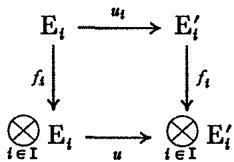
\includegraphics[keepaspectratio]{images/part003_14ac730d.jpg}}

是交换的，其中 \(f_{i}\) 和 \(f_{i}^{\prime}\) 表示典范同态。

只需将命题 8 应用于同态 \(f_{i}^{\prime} \circ u_{i}\) .

在命题 8 的推论中定义的同态 \(u\) 记作 \(\bigotimes_{i \in I} u_i\) 。若 \(J\) 是 \(I\) 的任意子集，则命题 8 可应用于典范同态族 \((f_i)_{i \in J}\) （诸 \(f_i: E_i \to \bigotimes_{i \in I} E_i = E\) ）；由此导出一个典范同态 \(E_J \to E\) ，它同样记作 \(f_J\) ，且当 \(J\) 有限时，它与上文中这样记的同态一致。

现在设 \((x_{i})_{i\in \mathbf{I}}\) 是 \(\prod_{i\in \mathbf{I}}\mathrm{E}_i\) 的一个元素，使得族 \((x_{i} - e_{i})_{i\in \mathbf{I}}\) 具有有限支撑 H。显然，若 J 和 \(J^{\prime}\) 是 I 的两个包含 H 的有限子集，则

\[
f _ {J} ((x _ {i}) _ {i \in J}) = f _ {J ^ {\prime}} ((x _ {i}) _ {i \in J ^ {\prime}}).
\]

 \(f_{\mathbf{J}}((x_i)_{i \in \mathbf{J}})\) （其中 \(\mathbf{J} \supset \mathbf{H}\) 遍历 \(\mathbf{I}\) 的有限子集）的公共值记为 \(\bigotimes_{i \in \mathbf{I}} x_i\) .

命题 9. 设 \((\mathbf{E}_i)_{i\in \mathbf{I}}\) 是一族 A-代数，且对每个 \(i\in \mathbf{I}\) ，设 \(B_{i}\) 是 \(\mathbf{E}_i\) 的一组基，使得单位元 \(e_i\) 属于 \(\overline{\mathbf{B}}_i\) 。设 \(\mathbf{B}\) 是形如 \(\bigotimes_{i\in \mathbf{I}}x_i\) 的元素组成的集合，其中 \((x_{i})\) 取遍 \(\prod_{i\in \mathbf{I}}\mathbf{B}_i\) 中使族 \((x_{i} - e_{i})\) 具有有限支撑的元素。则 \(\mathbf{B}\) 是代数 \(\bigotimes_{i\in \mathbf{I}}\mathbf{E}_i\) 的一组基，且这组基包含单位元 \(e\) .

对 I 的每个有限子集 J，设 \(B_{J}\) 是 \(E_{J} = \bigotimes_{i \in J} E_{i}\) 的基，即诸基 \(B_{i}\) （ \(i \in J\) ）的张量积（II, §3, 第 9 号）。由定义立即得出，B 是诸 \(f_{J}(B_{J})\) 当 J 遍历 \(\mathfrak{F}(I)\) 时的并，且 \(f_{J^{\prime}J}(B_{J}) \subset B_{J^{\prime}}\) 当 \(J \subset J^{\prime}\) 时成立；因此 \((B_{J})\) 是诸 \(E_{J}\) 的子集的一个正向系统，且 \(B = \varinjlim B_{J}\) ；结论由 II, §6, 第 2 号, 命题 5 的推论得出。

基 B 也称为诸基 \(B_{i}\) （ \(i \in I\) ）的张量积；当命题 9 的条件满足时，典范同态 \(f_{J}: E_{J} \to E = \bigotimes_{i \in I} E_{i}\) 对 I 的每个子集 J 都是单射，因为若 \(B_{J}\) 是 \(E_{J}\) 的基，即诸 \(B_{i}\) （ \(i \in J\) ）的张量积，则立即可以验证 \(f_{J}\) 在 \(B_{J}\) 上的限制是单射，且把 \(B_{J}\) 映到 B 的一个子集上。

\subsection{交换引理}

引理 1. 设 \(\mathbf{A}\) 是一个交换环， \(\mathbf{E}\) 是一个 \(\mathbf{A}\) -代数， \((x_{i})_{1\leqslant i\leqslant n}\) 是 \(\mathbf{E}\) 的元素组成的一个有限序列， \((\lambda_i)_{1\leqslant i\leqslant n}\) 是 \(\mathbf{A}\) 的元素组成的一个有限序列， \(y\) 是 \(\mathbf{E}\) 的一个元素；假设

\[
x _ {i} y = \lambda_ {i} y x _ {i} \quad \text { for } 1 \leqslant i \leqslant n.\tag{13}
\]

那么

\[
\left(x _ {1} x _ {2} \dots x _ {n}\right) y = \left(\lambda_ {1} \lambda_ {2} \dots \lambda_ {n}\right) y \left(x _ {1} x _ {2} \dots x _ {n}\right).\tag{14}
\]

该引理对 \(n = 1\) 是平凡的，我们对 \(n \geqslant 2\) 作归纳论证。现在

\[
\begin{array}{r l} (x _ {1} x _ {2} \dots x _ {n}) y & = (x _ {1} \dots x _ {n - 1}) (x _ {n} y) \\ & = (x _ {1} \dots x _ {n - 1}) (\lambda_ {n} y x _ {n}) = \lambda_ {n} ((x _ {1} \dots x _ {n - 1}) y) x _ {n}, \end{array}
\]

根据归纳假设，其等于

\[
\lambda_ {n} \left(\lambda_ {1} \dots \lambda_ {n - 1}\right) y \left(x _ {1} \dots x _ {n - 1}\right) x _ {n} = \left(\lambda_ {1} \dots \lambda_ {n - 1} \lambda_ {n}\right) y \left(x _ {1} \dots x _ {n - 1} x _ {n}\right),
\]

由此即得引理。

引理 2. 设 A 是一个交换环，E 是一个 A-代数， \((x_{i})_{1\leqslant i\leqslant n}\) 和 \((y_{i})_{1\leqslant i\leqslant n}\) 是 E 的由 \(n\) 个元素组成的两个有限序列；假设对 \(1\leqslant j\leqslant i\leqslant n\) ，

\[
x _ {i} y _ {j} = \lambda_ {i j} y _ {j} x _ {i} \quad \text { with } \lambda_ {i j} \in A.\tag{15}
\]

那么

\[
\left(x _ {1} x _ {2} \dots x _ {n}\right) \left(y _ {1} y _ {2} \dots y _ {n}\right) = \left(\prod_ {i > j} \lambda_ {i j}\right) \left(x _ {1} y _ {1}\right) \left(x _ {2} y _ {2}\right) \dots \left(x _ {n} y _ {n}\right).\tag{16}
\]

该引理对 \(n = 1\) 是平凡的，我们对 \(n\) （ \(n \geqslant 2\) ）再次作归纳论证。根据引理 1，

\[
\begin{array}{r l} (x _ {1} \dots x _ {n}) (y _ {1} \dots y _ {n}) & = x _ {1} (x _ {2} \dots x _ {n}) y _ {1} (y _ {2} \dots y _ {n}) \\ & = \left(\prod_ {i > 1} \lambda_ {i 1}\right) (x _ {1} y _ {1}) (x _ {2} \dots x _ {n}) (y _ {2} \dots y _ {n}) \end{array}
\]

然后只需应用归纳假设即可得到 (16)。

对元素的每个族 \(\lambda = (\lambda_{ij})\) （元素属于 A，且 \(1 \leqslant j < i \leqslant n\) ），以及对每个置换 \(\sigma \in \mathfrak{S}_n\) ，我们记

\[
\varepsilon_ {\sigma} (\lambda) = \prod_ {i > j, \sigma^ {- 1} (i) < \sigma^ {- 1} (j)} \lambda_ {i j} = \prod_ {i <   j, \sigma (i) > \sigma (j)} \lambda_ {\sigma (i), \sigma (j)}.\tag{17}
\]

注意，当 \(\mathbf{A} = \mathbf{Z}\) 且 \(\lambda_{ij} = -1\) 对每个有序对 \((i,j)\) （满足 \(1 \leqslant j < i \leqslant n\) ）成立时， \(\varepsilon_{\sigma}(\lambda)\) 就是符号 \(\varepsilon_{\sigma}\) （置换 \(\sigma\) 的符号）（I, §5, 第 7 号）。

引理 3. 设 A 是一个交换环，E 是一个 A-代数， \((x_{i})_{1\leqslant i\leqslant n}\) 是 E 的元素组成的一个有限序列，并假设对每个整数有序对 \((i,j)\) （满足 \(1\leqslant j < i\leqslant n\) ），

\[
x _ {i} x _ {j} = \lambda_ {i j} x _ {j} x _ {i} \quad \text { with } \lambda_ {i j} \in A.\tag{18}
\]

那么，对每个置换 \(\sigma \in \mathfrak{S}_n\) ，

\[
x _ {\sigma (1)} x _ {\sigma (2)} \dots x _ {\sigma (n)} = \varepsilon_ {\sigma} (\lambda) x _ {1} x _ {2} \dots x _ {n}.\tag{19}
\]

该引理对 \(n = 1\) 和 \(n = 2\) 是平凡的；我们对 \(n\) （ \(n \geqslant 3\) ）作归纳。若 \(\sigma(n) = n\) ，则关系式 (19) 由归纳假设得出。因此设 \(\sigma(n) = k, k \neq n\) ，并令 \(\tau\) 为 \([1, n]\) 上由下式定义的置换

\[
\left\{ \begin{array}{l l} \tau (i) = i & \text { for } i <   k \\ \tau (i) = i + 1 & \text { for } k \leqslant i <   n \\ \tau (n) = k. \end{array} \right.
\]

设 \(\pi = \tau^{-1} \circ \sigma\) ；置换 \(\pi\) 保持 \(n\) 不动；现在 \(\sigma = \tau \circ \pi\) ，因此，记 \(y_i = x_{\tau(i)}\) ，就有 \(y_{\pi(i)} = x_{\sigma(i)}\) 。若 \(i \neq n\) 且 \(j \neq n\) ，关系 \(\pi(i) > \pi(j)\) 与 \(\sigma(i) > \sigma(j)\) 等价（因为 \(\tau\) 是从 \([1, n - 1]\) 到 \([1, n]\) 的严格递增映射。对 \(i \neq n\) , \(j \neq n\) 和 \(\sigma(i) > \sigma(j)\) ，

\[
y _ {\pi (i)} y _ {\pi (j)} = x _ {\sigma (i)} x _ {\sigma (j)} = \lambda_ {\sigma (i), \sigma (j)} x _ {\sigma (j)} x _ {\sigma (i)} = \lambda_ {\sigma (i), \sigma (j)} y _ {\pi (j)} y _ {\pi (i)}
\]

因此，根据归纳假设（利用 \(\pi(n) = n\) ）:

\[
y _ {\pi (1)} y _ {\pi (2)} \dots y _ {\pi (n)} = \left(\prod_ {i <   j <   n, \sigma (i) > \sigma (j)} \lambda_ {\sigma (i), \sigma (j)}\right) y _ {1} y _ {2} \dots y _ {n}
\]

即

\[
x _ {\sigma (1)} x _ {\sigma (2)} \dots x _ {\sigma (n)} = \left(\prod_ {i <   j <   n, \sigma (i) > \sigma (j)} \lambda_ {\sigma (i), \sigma (j)}\right) x _ {\tau (1)} \dots x _ {\tau (n)}.\tag{20}
\]

现在

\[
x _ {\tau (1)} \dots x _ {\tau (n)} = x _ {1} \dots x _ {k - 1} x _ {k + 1} \dots x _ {n} x _ {k}
\]

而由引理 1，这等于

\[
\left(\prod_ {j > k} \lambda_ {j k}\right) x _ {1} \dots x _ {n} = \left(\prod_ {\sigma (i) > \sigma (n)} \lambda_ {\sigma (i), \sigma (n)}\right) x _ {1} \dots x _ {n}.\tag{21}
\]

最后，(20) 与 (21) 给出

\[
x _ {\sigma (1)} \dots x _ {\sigma (n)} = \alpha . x _ {1} \dots x _ {n}
\]

其中

\[
\begin{array}{l} \alpha = \left(\prod_ {i <   j <   n, \sigma (i) > \sigma (j)} \lambda_ {\sigma (i), \sigma (j)}\right) \cdot \left(\prod_ {i <   n, \sigma (i) > \sigma (n)} \lambda_ {\sigma (i), \sigma (n)}\right) \\ = \prod_ {i <   j, \sigma (i) > \sigma (j)} \lambda_ {\sigma (i), \sigma (j)} = \varepsilon_ {\sigma} (\lambda) \end{array}
\]

这就完成了引理 3 的证明。

\subsection{相对于交换因子的分次代数的张量积}

定义 6. 设 \((\Delta_{i})_{i\in I}\) 是一个以加法记号书写的交换幺半群的有限族。一个 \(\Delta_{i}\) 上的、取值于交换环 A 的交换因子系，是指一个映射系统 \(\varepsilon_{ij}:\Delta_i\times \Delta_j\to \mathbf{A}\) （其中 \(i\in \mathbf{I}, j\in \mathbf{I}, i\neq j\) ），满足以下条件：

\[
\varepsilon_ {i j} \left(\alpha_ {i} + \alpha_ {i} ^ {\prime}, \beta_ {j}\right) = \varepsilon_ {i j} \left(\alpha_ {i}, \beta_ {j}\right) \varepsilon_ {i j} \left(\alpha_ {i} ^ {\prime}, \beta_ {j}\right)\tag{22}
\]

\[
\varepsilon_ {i j} \left(\alpha_ {i}, \beta_ {j} + \beta_ {j} ^ {\prime}\right) = \varepsilon_ {i j} \left(\alpha_ {i}, \beta_ {j}\right) \varepsilon_ {i j} \left(\alpha_ {i}, \beta_ {j} ^ {\prime}\right)\tag{23}
\]

\[
\varepsilon_ {i j} (\alpha_ {i}, \beta_ {j}) \varepsilon_ {j i} (\beta_ {j}, \alpha_ {i}) = 1,\tag{24}
\]

对所有 \(\alpha_{i},\alpha_{i}^{\prime}\) （属于 \(\Delta_{i},\beta_{j},\beta_{j}^{\prime}\) ）以及 \(\Delta_j\) 中的元素成立。

若给 I 赋予一个全序且 \(\Delta_{i}\) 是群，则在 \(\Delta_{i}\) 上可以如下定义一个交换因子系：对每个有序对 \((i,j)\) （满足 i\textless j ），任取一个从 \(\Delta_{i}\times\Delta_{j}\) 到由环 A 的可逆元素组成的（乘法）Z-模 A* 的 Z-双线性映射，然后写出

\[
\varepsilon_ {j i} (\beta_ {j}, \alpha_ {i}) = (\varepsilon_ {i j} (\alpha_ {i}, \beta_ {j})) ^ {- 1}
\]

对 \(i < j\) .

注意，由于 \(\varepsilon_{ij}(\alpha_{i},\beta_{j})\) 都是可逆的，

\[
\varepsilon_ {i j} (0, \beta_ {j}) = \varepsilon_ {i j} (\alpha_ {i}, 0) = 1,
\]

由 (22) 与 (23) 即得。

例。(1) 平凡的交换因子系由满足下列条件的 \(\varepsilon_{ij}\) 组成： \(\varepsilon_{ij}(\alpha_i, \beta_j) = 1\) 对所有 \(i, j, \alpha_i \in \Delta_i, \beta_j \in \Delta_j\) 成立.

\begin{enumerate}
\def\labelenumi{(\arabic{enumi})}
\setcounter{enumi}{1}
\tightlist
\item
  若取 \(\mathbf{A} = \mathbf{Z}\) 且取 \(\Delta_{i} = \mathbf{Z}\) （对所有 \(i \in \mathbf{I}\) ），则令 \(\varepsilon_{ij}(\alpha_i, \beta_j) = (-1)^{\alpha_i\beta_j}\) 即得到一个交换因子系。注意，这个数仅依赖于 \(\alpha_{i}\) 和 \(\beta_{j}\) 的奇偶性，因此 \(\varepsilon_{ij}\) 在某些 \(\Delta_{i}\) 等于 \(\mathbf{Z}/2\mathbf{Z}\) 而其余的等于 \(\mathbf{Z}\) 的情形下仍可作为交换因子。
\end{enumerate}

这两个例子是应用中最常见的情况。

命题 10. 设 A 是一个交换环， \((\Delta_{i})_{i\in I}\) 是一个以加法记号书写的交换幺半群的有限族；对每个 \(i\in I\) ，设 \(\mathbf{E}_i\) 是一个类型为 \(\Delta_i\) 的分次 A-代数。最后，设 \((\varepsilon_{ij})\) 是 \(\Delta_i\) 上的一个取值于 A 的交换因子系。则存在一个类型为 \(\Delta = \prod_{i\in I}\Delta_i\) 的分次 A-代数 E，以及对每个 \(i\in I\) 的一个代数同态 \(h_i:\mathbf{E}_i\to \mathbf{E}\) ，具有下列性质：

\begin{enumerate}
\def\labelenumi{(\roman{enumi})}
\item
  若 \(\phi_{i}:\Delta_{i}\to\Delta\) 是典范同态，则 \(h_{i}\) 是分次同态（II, § 11, 第 2 号），换言之， \(h_{i}(E_{i}^{\alpha_{i}})\subset E^{\phi_{i}(\alpha_{i})}\) ，其中 \((E_{i}^{\alpha_{i}})\) 与 \((E^{\alpha})\) 分别表示 \(E_{i}\) 与 \(E\) 上的分次。
\item
  若 \(i \neq j\) 且 \(x_{i}\) （相应地 \(x_{j}\) ）是 \(\mathbf{E}_i\) （相应地 \(\mathbf{E}_j\) ）的次数为 \(\alpha_i \in \Delta_i\) （相应地 \(\beta_j \in \Delta_j\) ）的齐次元素，则
\end{enumerate}

\[
h _ {i} (x _ {i}) h _ {j} (x _ {j}) = \varepsilon_ {i j} (\alpha_ {i}, \beta_ {j}) h _ {j} (x _ {j}) h _ {i} (x _ {i}).\tag{25}
\]

\begin{enumerate}
\def\labelenumi{(\roman{enumi})}
\setcounter{enumi}{2}
\tightlist
\item
  对每个 A-代数 \(\mathbf{F}\) 以及每个满足下列条件的同态系统 \(f_{i}:\mathbf{E}_{i}\to \mathbf{F}\)
\end{enumerate}

\[
f _ {i} (x _ {i}) f _ {j} (x _ {j}) = \varepsilon_ {i j} (\alpha_ {i}, \beta_ {j}) f _ {j} (x _ {j}) f _ {i} (x _ {i}),\tag{26}
\]

其中 \(i, j, x_i, x_j, \alpha_i, \beta_j\) 如 (ii) 中所述，则存在且仅存在一个代数同态 \(f: \mathbf{E} \to \mathbf{F}\) ，使得 \(f_i = f \circ h_i\) 对所有 \(i \in \mathbf{I}\) 成立。此外， \(\mathbf{E}\) 的底 A-模是张量积 \(\bigotimes_{i \in \mathbf{I}} \mathbf{E}_i\) .

考虑 A-模 \(E = \bigotimes_{i \in I} E_i\) ；它等同于子模 \(E^\alpha\) 的直和，其中对每个 \(\alpha = (\alpha_i) \in \Delta\) ，记 \(E^\alpha = \bigotimes_{i \in I} E_i^{\alpha_i}\) ；因而这些 \(E^\alpha\) 在 A-模 E 上构成一个类型为 \(\Delta\) 的分次。我们将要在 E 上定义一个类型为 \(\Delta\) 的分次 A-代数结构。为此，给 I 一个全序；对每一对元素 \(\alpha = (\alpha_i)\) , \(\beta = (\beta_i)\) （属于 \(\Delta\) ），我们必须首先定义一个从 \(E^\alpha \times E^\beta\) 到 \(E^\alpha + \beta\) 的 A-双线性映射，或者等价地，定义一个 A-线性映射 \(m_{\alpha\beta}\) ，它把 \(E^\alpha \otimes_A E^\beta\) 映到 \(E^\alpha + \beta\) 。我们将用条件来定义 \(m_{\alpha\beta}\)

\[
m _ {\alpha \beta} \left(\left(\bigotimes_ {i \in I} x _ {i}\right) \otimes \left(\bigotimes_ {i \in I} y _ {i}\right)\right) = \varepsilon (\alpha , \beta) \bigotimes_ {i \in I} (x _ {i} y _ {i})\tag{27}
\]

对于 \(x_{i}\in \mathrm{E}_{i}^{\alpha_{i}},y_{i}\in \mathrm{E}_{i}^{\beta_{i}}\) ，其中

\[
\varepsilon (\alpha , \beta) = \prod_ {i > j} \varepsilon_ {i j} (\alpha_ {i}, \beta_ {j}).\tag{28}
\]

(27) 的右边显然属于 \(\mathbf{E}^{\alpha +\beta}\) ，且映射 \((x_{1},\ldots ,x_{n},y_{1},\ldots ,y_{n})\mapsto \varepsilon (\alpha ,\beta)\bigotimes_{i\in I}(x_{i}y_{i})\) 在诸 \(\mathrm{E}_i^{\alpha_i}\) 与诸 \(\mathrm{E}_i^{\beta_i}(1\leqslant i\leqslant n)\) 的乘积中是 A-多重线性的。接着必须证明这样定义在 E 上的乘法是结合的；现在，若 \(\gamma = (\gamma_{i})\) 是 \(\Delta\) 的第三个元素，且 \(z_{i} \in \mathrm{E}_{i}^{\gamma_{i}}\) （对 \(1 \leqslant i \leqslant n\) ），则

\[
\left(\left(\bigotimes_ {i} x _ {i}\right) \left(\bigotimes_ {i} y _ {i}\right)\right) \left(\bigotimes_ {i} z _ {i}\right) = \varepsilon (\alpha + \beta , \gamma) \varepsilon (\alpha , \beta) \bigotimes_ {i} (x _ {i} y _ {i} z _ {i})
\]

\[
\left(\bigotimes_ {i} x _ {i}\right) \left(\left(\bigotimes_ {i} y _ {i}\right) \left(\bigotimes_ {i} z _ {i}\right)\right) = \varepsilon (\alpha , \beta + \gamma) \varepsilon (\beta , \gamma) \bigotimes_ {i} (x _ {i} y _ {i} z _ {i})
\]

从而只需验证恒等式

\[
\varepsilon (\alpha + \beta , \gamma) \varepsilon (\alpha , \beta) = \varepsilon (\alpha , \beta + \gamma) \varepsilon (\beta , \gamma).
\]

但后者立即由以下关系得出

\[
\varepsilon (\alpha + \beta , \gamma) = \varepsilon (\alpha , \beta) \varepsilon (\beta , \gamma)
\]

\[
\varepsilon (\alpha , \beta + \gamma) = \varepsilon (\alpha , \beta) \varepsilon (\alpha , \gamma)
\]

这些关系本身是定义(28)、(22)和(23)的直接推论。

若对所有 \(i \in \mathbf{I}\) ， \(e_i\) 表示 \(\mathbf{E}_i\) 的单位元，我们知道 \(e_i\) 是 0 次齐次的（§ 3, 第 1 号），因此 \(e = \bigotimes_{i \in \mathbf{I}} e_i\) 是 0 次齐次的，并且由 (27)、(28) 及关系式

\[
\varepsilon_ {i j} (\alpha_ {i}, 0) = \varepsilon_ {i j} (0, \beta_ {j}) = 1
\]

即 \(e\) 是 \(\mathbf{E}\) 的单位元，这就完成了 \(\mathbf{E}\) 上所需要的分次 A-代数结构的定义。然后取 \(h_i(x_i) = x_i \otimes \bigotimes_{j \neq i} e_j\) ；为验证 \(h_i(x_i x_i') = h_i(x_i) h_i(x_i')\) 对 \(x_i, x_i'\) （属于 \(\mathbf{E}_i\) ）成立，只需限于 \(x_i\) 和 \(x_i'\) 均为齐次元素的情形，此时该关系由 (27) 和关系式 \(\varepsilon_{ij}(\alpha_i, 0) = \varepsilon_{ij}(0, \beta_j) = 1\) 立即得出；同样的关系式以及 (24) 还证明了 \(h_i\) 满足命题中的条件 (i) 与 (ii)，且

\[
\bigotimes_ {i \in I} x _ {i} = \prod_ {i \in I} h _ {i} (x _ {i})\tag{29}
\]

其中右端是有序序列 \((h_i(x_i))_{i\in I}\) 按 I 上给定的全序在 E 中取的乘积（I, § 1, 第 2 号）（只需对 \(x_{i}\) （设为齐次）中异于 \(e_i\) 者的个数作归纳论证即可）.

仍需证明条件 (iii)；注意，映射

\[
(x _ {i}) _ {i \in I} \mapsto \prod_ {i \in I} f _ {i} (x _ {i}),
\]

其中右端是有序序列 \((f_{i}(x_{i}))_{i\in\mathbf{I}}\) 按 I 上给定的全序取的乘积，是 A-多重线性的。于是存在且仅存在一个 A-线性映射 \(f: E \rightarrow F\) ，使得

\[
f \left(\bigotimes_ {i \in I} x _ {i}\right) = \prod_ {i \in I} f _ {i} (x _ {i}).\tag{30}
\]

显然 \(f(e)\) 是 \(\mathbf{F}\) 的单位元，且 \(f \circ h_i = f_i\) ；为验证 \(f\) 是代数同态，换言之，验证 \(f(x)f(y) = f(xy)\) 对 \(x, y\) （属于 \(\mathbf{E}\) ）成立，由线性性，只需限于下列情形： \(x = \bigotimes_{i \in \mathbf{I}} x_i\) 且 \(y = \bigotimes_{i \in \mathbf{I}} y_i\) ，其中 \(x_i\) （相应地 \(y_i\) ）是次数为 \(\alpha_i\) （相应地 \(\beta_i\) ）的齐次元素（对所有 \(i \in \mathbf{I}\) ）。此时，要验证的关系式由 (27) 化归为

\[
\left(\prod_ {i \in \mathrm{I}} f _ {i} (x _ {i})\right) \left(\prod_ {i \in \mathrm{I}} f _ {i} (y _ {i})\right) = \varepsilon (\alpha , \beta) \prod_ {i \in \mathrm{I}} \left(f _ {i} (x _ {i}) f _ {i} (y _ {i})\right).
\]

但考虑到关系式 (26)，这是第 6 号的引理 2 的一个推论。

显然，代数 E 与典范映射 \(\psi: \bigotimes_{i \in I} E_i \to E\) 构成泛映射问题（集合论, IV, § 3, 第 1 号）的一个解，其中 \(\Sigma\) 是 A-代数结构的种类，而 \(\alpha\) -映射是映射 \(\prod_{i} f_i\) （从 \(\prod_{i} E_i\) 到一个 A-代数，满足条件 (26)）。

对 I 上固定的一个全序，命题 10 的证明中所定义的分次代数 E 将称为一个分次张量 \(\varepsilon\) -积，其类型为 \(\Delta\) ，所属的族为 \((\mathrm{E}_i)_{i\in \mathbf{I}}\) （族中各代数的类型为 \(\Delta_i\) ），并记作 \({}^{\varepsilon}\bigotimes_{i\in \mathbf{I}}\mathrm{E}_i\) （若关于 I 上的序不致引起混淆）；类似地，命题 10 的证明中定义的同态 \(f:\mathrm{E}\to \mathrm{F}\) 将记作 \({}^{\varepsilon}\bigotimes_{i\in \mathbf{I}}f_i\) 。同态 \(h_i\) 称为典范的。我们也写作 \({}^{\varepsilon}\mathrm{G}^{\otimes n}\) （当 \(\mathbf{I} = [1,n]\) 且所有 \(\mathrm{E}_i\) 都等于同一个代数 G 时）。

注。(1) 若取 \(\varepsilon_{ij}(\alpha_i, \beta_j) = 1\) （对所有 \(i, j, \alpha_i\) 与 \(\beta_j\) ），我们就重新得到第 1 号中定义的代数的张量积（其分次还是各因子的分次的张量积）.

\begin{enumerate}
\def\labelenumi{(\arabic{enumi})}
\setcounter{enumi}{1}
\tightlist
\item
  设所有 \(\Delta_{i}\) 都等于 \(\mathbf{Z}\) ，并写 \(\varepsilon_{ij}(\alpha_i, \beta_j) = (-1)^{\alpha_i \beta_j}\) ；对应于这个交换因子系的张量 \(\varepsilon\) -积 \({}^{\varepsilon}\bigotimes_{i \in I} E_i\) 称为分次代数 \(E_i\) （类型为 \(\mathbf{Z}\) ）的斜张量积，记作 \({}^{g}\bigotimes_{i \in I} E_i\) （对两个代数则记 \(E{}^{g} \otimes_A F\) ，或以 \({}^{g} G^{\otimes n}\) 代替 \({}^{\varepsilon} G^{\otimes n}\) ）.
\end{enumerate}

推论 1. 在命题 10 的记号下，进一步设 F 是一个类型为 \(\Delta\) 的分次 A-代数，且每个 \(f_{i}\) 都是相对于 \(\phi_{i}:\Delta_{i}\to\Delta\) 的分次代数同态；则 \(f={}^{\varepsilon}\bigotimes_{i}f_{i}\) 是一个分次代数同态。

这由 \(f\) 的定义以及下列事实立即得出：

\[
\sum_ {i \in I} \phi_ {i} (\alpha_ {i}) = (\alpha_ {i})
\]

这是由 \(\phi_{i}\) 的定义得到的.

由此可以看出， \((\mathrm{E},\psi)\) 也是另一个泛映射问题的解，这一次 \(\Sigma\) 是类型为 \(\Delta\) 的分次 A-代数结构的种类，其态射是类型为 \(\Delta\) 的分次代数同态，而 \(\alpha\) -映射是映射 \(\prod_{i}f_{i}\) （其中除条件 (26) 外，还假设 \(f_{i}\) 是相对于 \(\phi_{i}\) 的分次代数同态）.

推论 2. 设 \((\mathbf{E}_i)_{i\in \mathbf{I}}\) , \((\mathbf{F}_i)_{i\in \mathbf{I}}\) 是两个有限的 A-代数族，且 \(\mathbf{E}_i\) 与 \(\mathbf{F}_i\) 都是类型为 \(\Delta_i\) 的分次代数（对所有 \(i\in \mathbf{I}\) ）。对每个 \(i\in \mathbf{I}\) ，设 \(g_i:\mathbf{E}_i\to \mathbf{F}_i\) 是一个类型为 \(\Delta_i\) 的分次代数同态。那么，若 \(h_i:\mathbf{E}_i\to {}^{\varepsilon}\bigotimes_{i\in \mathbf{I}}\mathbf{E}_i\) 与 \(h_i':\mathbf{F}_i\to {}^{\varepsilon}\bigotimes_{i\in \mathbf{I}}\mathbf{F}_i\) 是典范同态，则存在且仅存在一个类型为 \(\Delta\) 的分次 A-代数同态 \(g: {}^{\varepsilon}\bigotimes_{i\in \mathbf{I}}\mathbf{E}_i\to {}^{\varepsilon}\bigotimes_{i\in \mathbf{I}}\mathbf{F}_i\) ，使得 \(g\circ h_i = h_i'\circ g_i\) 对所有 \(i\in \mathbf{I}\) 成立。此外，若每个 \(g_i\) 都是双射，则 \(g\) 也是.

只需将推论 1 应用于 \(f_{i} = h_{i}^{\prime} \circ g_{i}\) ，并注意到条件 (26) 可由应用于 \(h_{i}^{\prime}\) 的关系式 (25) 得出。

推论 2 中定义的同态也记作 \({}^{\varepsilon}\bigotimes_{i} g_{i}\) （若不致引起混淆）；若对每个 \(i \in I\) ， \(G_{i}\) 是又一个分次 A-代数（类型为 \(\Delta_{i}\) ），且 \(g_{i}^{\prime}: F_{i} \to G_{i}\) 是一个分次代数同态，则

\[
\left(^ {\varepsilon} \bigotimes_ {i} g _ {i} ^ {\prime}\right) \circ \left(^ {\varepsilon} \bigotimes_ {i} g _ {i}\right) = ^ {\varepsilon} \bigotimes_ {i} \left(g _ {i} ^ {\prime} \circ g _ {i}\right),\tag{31}
\]

这由(30)立即得出。

在斜张量积（类型为 \(\mathbf{Z}\) 的分次代数的）情形，我们写 \({}^{g}\bigotimes_{i}f_{i}\) 以代替 \({}^{\varepsilon}\bigotimes_{i}f_{i}\) ——对同态 \(f_{i}: \mathrm{E}_{i} \to \mathrm{F}_{i}\) （类型为 \(\mathbf{Z}\) 的分次代数的同态）而言；当 \(\mathrm{I} = \{1, 2\}\) 时，这个同态也记作 \(f_{1}{}^{g}\otimes f_{2}\) ；当 \(\mathrm{I} = [1, n]\) 且所有 \(\mathrm{E}_{i}\) （相应地 \(\mathrm{F}_{i}\) ）相等并且所有 \(f_{i}\) 都等于同一个同态 \(f\) 时，我们写 \({}^{g}f^{\otimes n}\) .

注。在命题 10 的证明中，I 上的一个全序被用来在张量积 \(\bigotimes_{i\in I}E_i\) 上定义一个代数结构，该张量积是 A-模

\(E_{i}\) 的张量积。若改变 I 上的序，则在 \(\bigotimes_{i\in I}E_{i}\) 上会产生另一个乘法结构，但这样得到的新代数与上述代数典范同构，因为二者都是同一个泛映射问题的解。例如，当 \(I=\{1,2\}\) 时，从代数 \(E_{1}{}^{\varepsilon}\otimes_{A}E_{2}\) 到代数 \(E_{2}{}^{\varepsilon}\otimes_{A}E_{1}\) 的典范同构把 \(x_{1}\otimes x_{2}\) 映为 \(\varepsilon_{2,1}(\alpha,\beta)x_{2}\otimes x_{1}\) ，其中 \(x_{1}\) 是次数为 \(\alpha\) 的齐次元素， \(x_{2}\) 是次数为 \(\beta\) 的齐次元素.

设 J 是 I 的一个子集，且对每个 \(i \in J\) ，考虑典范同态 \(h_{i}: E_{i} \to {}^{\varepsilon}\bigotimes_{i \in I} E_{i} = E\) 。借助关系式 (25)，从这些同态典范地（由命题 10）导出一个典范同态 \(h: E' = {}^{\varepsilon}\bigotimes_{i \in J} E_{i} \to E\) ，使得对所有 \(i \in J\) ， \(h_{i}' = h \circ h_{i}\) ，其中 \(h_{i}'\) 是典范同态 \(E_{i} \to E'\) 。取 J 上由 I 上所选的全序诱导的全序，我们得到

\[
h \left(\bigotimes_ {i \in J} x _ {i}\right) = \prod_ {i \in I} h _ {i} \left(x _ {i}\right) = \bigotimes_ {i \in I} x _ {i} ^ {\prime}
\]

其中中间项是有序序列 \((h_i(x_i))_{i\in J}\) 的乘积，而在右端项中， \(x_{i}^{\prime} = x_{i}\) 对 \(i\in J\) 成立， \(x_{i}^{\prime} = e_{i}\) 对 \(i\notin J\) 成立.

命题 11.（张量 \(\varepsilon\) -积的“结合性”）。在命题 10 的记号下，设 \((J_{\lambda})_{\lambda \in L}\) 是 I 的一个划分，并记 \(\Delta_{\lambda}' = \prod_{i \in J_{\lambda}} \Delta_i\) （对所有 \(\lambda \in L\) ）。设 \(E_{\lambda}'\) 是一个分次张量 \(\varepsilon\) -积，其类型为 \(\Delta_{\lambda}'\) ，所属的族为 \((E_i)_{i \in J_{\lambda}}\) （对 \(J_{\lambda}\) 上选定的某个全序而言）。另一方面，对 L 中的 \(\lambda, \mu\) 且 \(\lambda \neq \mu\) ，我们对 \(\alpha_{\lambda}' = (\alpha_i)_{i \in J_{\lambda}}, \beta_{\mu}' = (\beta_j)_{j \in J_{\mu}}\) 写

\[
\varepsilon_ {\lambda \mu} ^ {\prime} (\alpha _ {\lambda} ^ {\prime}, \beta_ {\mu} ^ {\prime}) = \prod_ {i \in J _ {\lambda}, j \in J _ {\mu}} \varepsilon_ {i j} (\alpha_ {i}, \beta_ {j}).\tag{32}
\]

那么 \((\varepsilon_{\lambda \mu}^{\prime})\) 是 \(\Delta_{\lambda}^{\prime}\) 上的一个取值于 A 的交换因子系，且存在且仅存在一个类型为 \(\Delta, v: {}^{\varepsilon'}\bigotimes_{\lambda \in L} E_{\lambda}^{\prime} \to {}^{\varepsilon}\bigotimes_{i \in I} E_{i}\) 的分次代数同态，使得

\[
v \left(\bigotimes_ {\lambda \in L} \left(\bigotimes_ {i \in J _ {\lambda}} x _ {i}\right)\right) = \bigotimes_ {i \in I} x _ {i}\tag{33}
\]

对所有 \((x_{i})\in \prod_{i\in \mathbf{I}}\mathrm{E}_{i}\) 成立，前提是在 \(\mathbf{I}\) 上取这样的全序：它在每个 \(\mathbf{J}_{\lambda}\) 上诱导所选的全序，并且使得对 \(\lambda < \mu\) （在 \(\mathbf{L}\) 中）、 \(i\in \mathbf{J}_{\lambda}\) 与 \(j\in \mathbf{J}_{\mu}\) ，有 \(i < j\) .

\(\varepsilon_{\lambda \mu}'\) 构成交换因子系这一事实是平凡的。设 \(h_{i,\lambda}:\mathrm{E}_i\to \mathrm{E}_{\lambda}', h_{\lambda}':\mathrm{E}_{\lambda}'\to {}^{\varepsilon'}\bigotimes_{\lambda \in L}\mathrm{E}_{\lambda}'\) 是典范同态（对 \(\lambda \in L\) , \(i\in \mathbf{J}_{\lambda}\) ），并记 \(h_i'' = h_\lambda' \circ h_{i,\lambda}\) ；由泛映射问题解的唯一性，只需证明 \({}^{\varepsilon'}\bigotimes_{\lambda \in L} E_{\lambda}'\) 与诸 \(h_i''\) 满足命题 10 的条件即可。现在，对所有 \(\lambda \in L\) ，设 \(f_{\lambda}': E_{\lambda}' \to F\) 是唯一的代数同态，使得 \(f_{\lambda}' \circ h_{i,\lambda} = f_i\) 对所有 \(i \in J_{\lambda}\) 成立。我们证明，对 \(\lambda \neq \mu\) , \(\alpha_{\lambda}' = (\alpha_i)_{i \in J_{\lambda}}\) , \(\beta_{\mu}' = (\beta_j)_{j \in J_{\mu}}\) ,

\[
f _ {\lambda} ^ {\prime} (x _ {\lambda} ^ {\prime}) f _ {\mu} ^ {\prime} (x _ {\mu} ^ {\prime}) = \varepsilon_ {\lambda \mu} ^ {\prime} (\alpha_ {\lambda} ^ {\prime}, \beta_ {\mu} ^ {\prime}) f _ {\mu} ^ {\prime} (x _ {\mu} ^ {\prime}) f _ {\lambda} ^ {\prime} (x _ {\lambda} ^ {\prime})\tag{34}
\]

对齐次元素 \(x_{\lambda}^{\prime} \in \mathrm{E}_{\lambda}^{\prime}\) （相应地 \(x_{\mu}^{\prime} \in \mathrm{E}_{\mu}^{\prime}\) ），其次数为 \(\alpha_{\lambda}^{\prime}\) （相应地 \(\beta_{\mu}^{\prime}\) ）；由线性性，只需在 \(x_{\lambda}^{\prime} = \bigotimes_{i \in J_{\lambda}} x_{i}\) , \(x_{\mu}^{\prime} = \bigotimes_{j \in J_{\mu}} x_{j}\) 的情形验证，其中 \(x_{i}\) （相应地 \(x_{j}\) ）是次数为 \(\alpha_{i}\) （相应地 \(\beta_{j}\) ）的齐次元素，属于 \(E_{i}\) （相应地 \(E_{j}\) ）（对 \(i \in J_{\lambda}, j \in J_{\mu}\) ）。但这由定义诸 \(f_{\lambda}^{\prime}\) 的公式 (30) 以及第 6 号的引理 3 得出，其中用到假设 (26) 与定义 (32)。因此存在且仅存在一个代数同态 \(f: ^{\varepsilon'} \bigotimes_{\lambda \in L} E_{\lambda}' \to F\) ，使得 \(f \circ h_{\lambda}' = f_{\lambda}'\) 对所有 \(\lambda \in L\) 成立；由此 \(f \circ h_{i}' = f_{i}\) 对所有 \(i \in I\) 成立，而 \(f\) 的唯一性是平凡的。

\subsection{同类型分次代数的张量积}

在第 7 号命题 10 的假设成立的前提下，进一步设所有 \(\Delta_{i}\) 都等于同一个交换幺半群 \(\Delta_{0}\) ；于是我们可以在张量 \(\varepsilon\) -积 \({}^{\varepsilon}\bigotimes_{i\in I}E_{i}\) 上考虑类型为 \(\Delta_{0}\) 的总分次，它与此代数上类型为 \(\Delta = \Delta_{0}^{I}\) 的分次相关联（II, § 11, 第 1 号）；我们将带有这个分次的 \({}^{\varepsilon}\bigotimes_{i\in I}E_{i}\) 称为一个分次张量 \(\varepsilon\) -积，其类型为 \(\Delta_{0}\) ，所属的族为 \((E_{i})_{i\in I}\) （族中各代数的类型为 \(\Delta_{0}\) ）.

保持第 7 号命题 10 的记号，设 F 也是一个类型为 \(\Delta_0\) 的分次 A-代数，且诸 \(f_i\) 是类型为 \(\Delta_0\) 的分次代数同态。则 \(f: {}^{\varepsilon}\bigotimes_{i \in I} E_i \to F\) 也是类型为 \(\Delta_0\) 的分次代数同态：因为由公式 (30)（第 7 号）可知，若 \(x_i\) 是齐次的且次数为 \(\alpha_i \in \Delta_0\) ，则 \(\bigotimes_{i \in I} x_i\) 与 \(\prod_{i \in I} f_i(x_i)\) 都是次数为 \(\sum_{i \in I} \alpha_i \in \Delta_0\) 的齐次元素.

因此可以说， \(\bigotimes_{i\in I}E_i\) （带有类型为 \(\Delta_0\) 的总分次）与典范映射 \(\psi\) 一起构成第三个泛映射问题的一个解，其中 \(\Sigma\) 是类型为 \(\Delta_0\) 的分次 A-代数的种类，态射是类型为 \(\Delta_0\) 的分次代数同态，而 \(\alpha\) -映射是映射 \(\prod_{i}f_{i}\) （其中除条件 (26)（第 7 号）外，还假设每个 \(f_{i}\) 是类型为 \(\Delta_0\) 的分次代数同态）.

对 I 的每个子集 J，典范同态 \({}^{\varepsilon}\bigotimes_{i\in J}E_i\to {}^{\varepsilon}\bigotimes_{i\in I}E_i\) （第 7 号）实际上是一个类型为 \(\Delta_0\) 的分次代数同态，这由上述内容立即得出。

命题 12.（同类型分次代数的张量 \(\varepsilon\) -积的“结合性”）。采用第 7 号命题 10 的记号，设所有 \(\Delta_{i}\) 都等于同一个幺半群 \(\Delta_{0}\) ；设 \((J_{\lambda})_{\lambda \in L}\) 是 I 的一个划分。采用第 7 号命题 11 的记号，设公式 (32)（第 7 号）的右端只依赖于和 \(\alpha_{\lambda}^{\prime \prime} = \sum_{i \in J_{\lambda}} \alpha_{i}, \beta_{\mu}^{\prime \prime} = \sum_{j \in J_{\mu}} \beta_{j}\) ——对相异指标的每个有序对 \((\lambda, \mu)\) 、所有 \(\alpha_{\lambda}^{\prime} \in \Delta_{\lambda}^{\prime}\) 以及所有 \(\beta_{\mu}^{\prime} \in \Delta_{\mu}^{\prime}\) 而言；令 \(\varepsilon_{\lambda \mu}^{\prime \prime}(\alpha_{\lambda}^{\prime \prime}, \beta_{\mu}^{\prime \prime})\) 表示 (32) 的右端。则 \((\varepsilon_{\lambda \mu}^{\prime \prime})\) 是族 \((\Delta_{\lambda}^{\prime \prime})_{\lambda \in L}\) 上的一个交换因子系，其中 \(\Delta_{\lambda}^{\prime \prime} = \Delta_{0}\) （对所有 \(\lambda \in L\) ）。若 \(E_{\lambda}^{\prime \prime}\) 是一个分次张量 \(\varepsilon\) -积，其类型为 \(\Delta_{0}\) ，所属的族为 \((E_{i})_{i \in J_{\lambda}}\) ，则存在且仅存在一个类型为 \(\Delta_{0}\) 的分次代数同构 \(w: {}^{\varepsilon}\bigotimes_{\lambda \in L} E_{\lambda}^{\prime \prime} \to {}^{\varepsilon}\bigotimes_{i \in I} E_{i}\) ，使得

\[
w \left(\bigotimes_ {\lambda \in L} \left(\bigotimes_ {i \in J _ {\lambda}} x _ {i}\right)\right) = \bigotimes_ {i \in I} x _ {i}\tag{35}
\]

前提是按第 7 号命题 11 所述，在 \(\mathbf{J}_{\lambda}\) 与 \(\mathbf{I}\) 上选取全序。

根据假设，对 \(\gamma\) , \(\delta\) （属于 \(\Delta_0\) ），有 \(\varepsilon_{\lambda \mu}''(\gamma, \delta) = \varepsilon_{i_0 j_0}(\gamma, \delta)\) （对某个 \(i_0 \in J_\lambda\) 与某个 \(j_0 \in J_\mu\) ），这可以通过考虑元素 \(\alpha_\lambda' = (\alpha_i)_{i \in J_\lambda}\) 与 \(\beta_\mu' = (\beta_j)_{j \in J_\mu}\) 看出，它们满足 \(\alpha_{i_0} = \gamma\) , \(\alpha_i = 0\) （对 \(i \neq i_0\) ）, \(\beta_{j_0} = \delta\) , \(\beta_j = 0\) （对 \(j \neq j_0\) ）；由此立即得出，诸 \(\varepsilon_{\lambda \mu}''\) 构成一个交换因子系。证明的其余部分与命题 11（第 7 号）的证明类似，留给读者完成。

注意，当 \(\Delta_0 = \mathbf{Z}\) 且 \((\varepsilon_{ij})\) 是平凡的因子系 \((\varepsilon_{ij}(\alpha_i,\beta_j) = 1\) 对所有 \(i,j)\) ，或是由 \(\varepsilon_{ij}(\alpha_i,\beta_j) = (-1)^{\alpha_i\beta_j}\) 定义的因子系时，命题 12 的附加假设成立；在后一情形，公式 (32) 的右端等于 \((-1)^{\gamma}\) ，其中 \(\gamma = \sum_{i\in J_{\lambda},j\in J_{\mu}}\alpha_{i}\beta_{j} = \left(\sum_{i\in J_{\lambda}}\alpha_{i}\right)\left(\sum_{j\in J_{\mu}}\beta_{j}\right)\) .

注。(1) 设 I 是一个无限指标集， \(\Delta_0\) 是一个交换幺半群；设 \((\Delta_i)_{i \in I}\) 表示满足 \(\Delta_i = \Delta_0\) （对所有 \(i\) ）的族，并对 I 的每对相异指标 \((i,j)\) 给定一个满足条件 (22)、(23) 与 (24)（第 7 号）的映射 \(\varepsilon_{ij} : \Delta_i \times \Delta_j \to A\) ；这也称为族 \((\Delta_i)\) 上的一个交换因子系。考虑一个族 \((E_i)_{i \in I}\) （由类型为 \(\Delta_0\) 的分次 A-代数组成）；对 I 的每个有限子集 J，令 \(E_J\) 表示一个分次张量 \(\varepsilon\) -积，其类型为 \(\Delta_0\) ，所属的子族为 \((E_i)_{i \in J}\) （对 J 上的全序作任意选取）。若 J 与 \(J'\) 是 I 的两个有限子集且 \(J \subset J'\) ，则上面已定义了一个类型为 \(\Delta_0\) 的分次代数的典范同态 \(h_{J^{\prime}J}:E_{J}\to E_{J^{\prime}}\) ，而这些同态的唯一性性质立即表明：若 \(J\subset J^{\prime}\subset J^{\prime\prime}\) 是 I 的三个有限子集，则 \(h_{J^{\prime\prime}J}=h_{J^{\prime\prime}J^{\prime}}\circ h_{J^{\prime}J}\) 。于是有一个正向系统 \((E_{J},h_{J^{\prime}J})\) ——由类型为 \(\Delta_{0}\) 的分次代数组成（§3, 第 3 号）——其指标集是 I 的有限子集组成的右有向集 \(\mathfrak{F}(I)\) 。类型为 \(\Delta_{0}\) 的分次代数——这个正向系统的正向极限（§3, 第 3 号）——称为一个分次张量 \(\varepsilon\) -积，其类型为 \(\Delta_{0}\) ，所属的族为 \((E_{i})_{i\in I}\) ；它也记作 \({}^{\varepsilon}\bigotimes_{i\in I}E_{i}\) 。当所有 \(\Delta_{i}\) 都等于 \(\mathbf{Z}\) 且 \(\varepsilon_{ij}(\alpha_{i},\beta_{j})=(-1)^{\alpha_{i}\beta_{j}}\) 时，张量积 \({}^{\varepsilon}\bigotimes_{i\in I}E_{i}\) 也称为

族 \((\mathbf{E}_{i})_{i\in\mathbb{I}}\) 的斜张量积，记作 \({}^{g}\bigotimes_{i\in I}E_{i}\) 。我们把如下命题的表述与证明留给读者：该命题把第 7 号的命题 10 推广到 I 为无限的情形，正如第 5 号的命题 8 把第 2 号的命题 5 推广到 I 为无限的情形那样。注意， \({}^{\varepsilon}\bigotimes_{i\in I}E_{i}\) 的底 A-模与第 5 号中定义的非分次代数的族 \((\mathbf{E}_{i})_{i\in\mathbb{I}}\) 的（非分次）张量积的底 A-模相同。

\begin{enumerate}
\def\labelenumi{(\arabic{enumi})}
\setcounter{enumi}{1}
\tightlist
\item
  设 E 是一个类型为 \(\Delta_0\) 的分次 A-代数（其中 \(\Delta_0\) 是一个交换幺半群），且 \(\rho: \mathbf{A} \to \mathbf{B}\) 是一个环同态； \(\rho^*(\mathbf{E})\) 上的分次（II, §11, 第 5 号）与分次张量积 \(\mathbf{B} \otimes_{\mathbf{A}} \mathbf{E}\) （其中 B 带有平凡分次）上的分次相同。
\end{enumerate}
